\input{../utils/preamble}
\createdgmtitle{8}
%--------------------------------------------------------------------------------
\begin{document}
%--------------------------------------------------------------------------------
\begin{frame}
%\thispagestyle{empty}
\titlepage
\end{frame}
%=======
\begin{frame}{Recap of previous lecture}
	Images are discrete datam flow is a continuous model.
	We need to convert a discrete data distribution to a continuous on.
	
	\begin{block}{Uniform dequantization bound}
		\vspace{-0.5cm}
		\[
			\bx \sim \text{Categorical}(\bpi), \quad 
			\bu \sim U[0, 1], \quad 
			\by = \bx + \bu \sim \text{Continuous} 
		\]
		\vspace{-0.4cm}
		\[
			\log P(\bx | \btheta) \geq \int_{U[0, 1]} \log p(\bx + \bu | \btheta) d \bu.
		\]
	\end{block}
	\vspace{-0.2cm}
	\begin{block}{Variational dequantization bound}
		Introduce variational dequantization noise distribution $q(\bu | \bx)$ and treat it as an approximate posterior. 
		\vspace{-0.2cm}
		\[
			\log P(\bx | \btheta) \geq  \int q(\bu | \bx) \log \frac{p(\bx + \bu | \btheta)}{q(\bu | \bx)} d \bu = \mathcal{L}(q, \btheta).
		\]
	\end{block}
	\myfootnotewithlink{https://arxiv.org/abs/1902.00275}{Ho J. et al. Flow++: Improving Flow-Based Generative Models with Variational Dequantization and Architecture Design, 2019}
\end{frame}
%=======
\begin{frame}{Recap of previous lecture}
	
	\begin{minipage}[t]{0.5\columnwidth}
		\begin{figure}
			\centering
			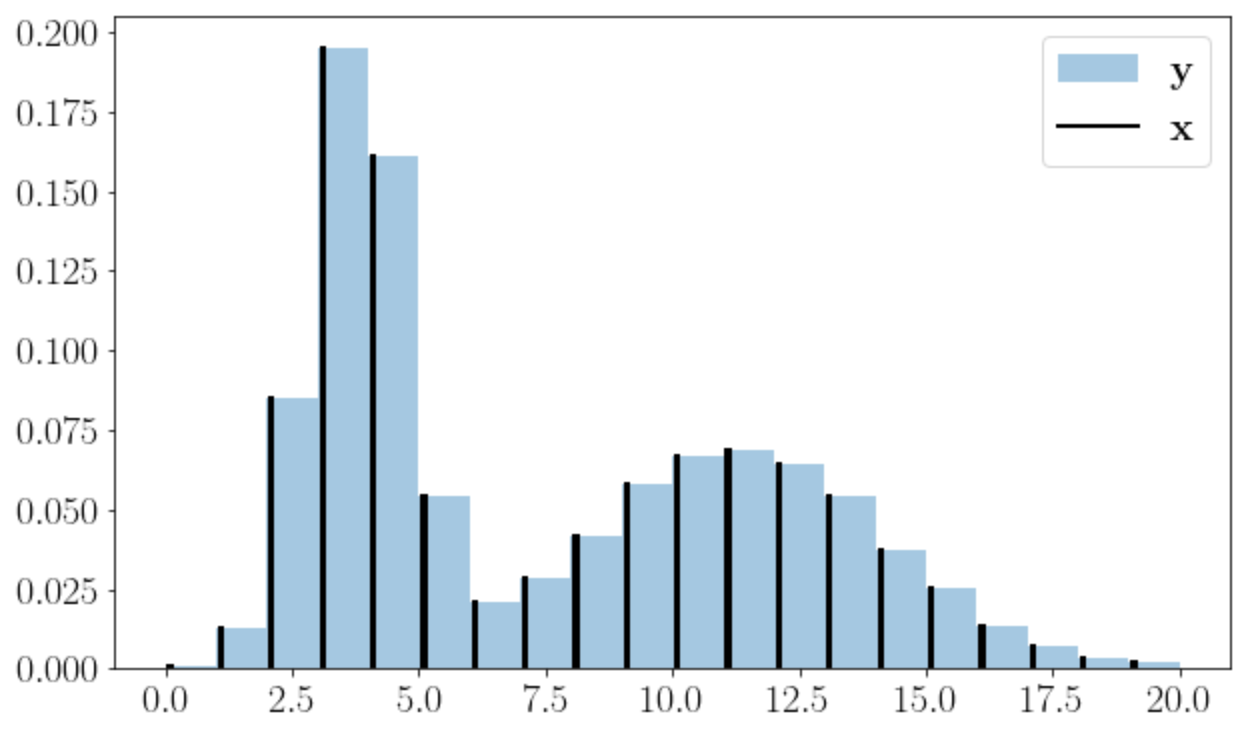
\includegraphics[width=1.0\linewidth]{figs/uniform_dequantization.png}
		\end{figure}
	\end{minipage}%
	\begin{minipage}[t]{0.5\columnwidth}
		\begin{figure}
			\centering
			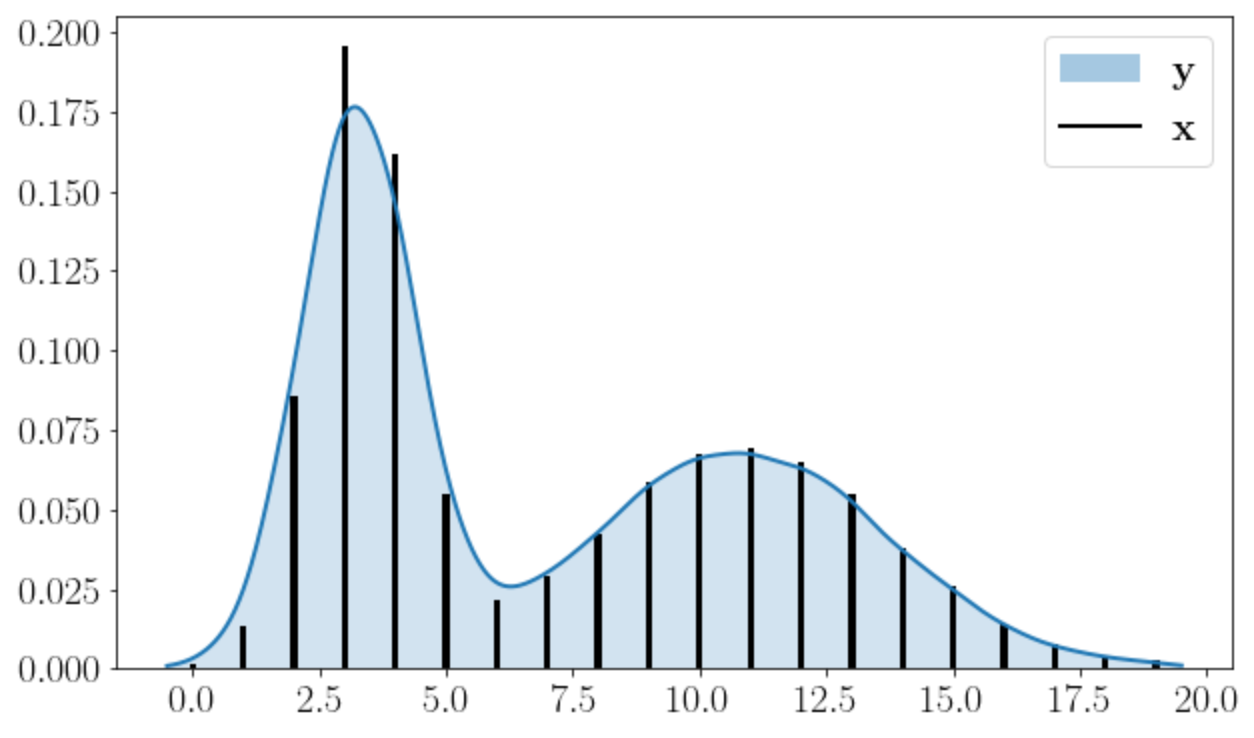
\includegraphics[width=1.0\linewidth]{figs/variational_dequantization.png}
		\end{figure}
	\end{minipage}
	\begin{block}{Flow model for dequantization}
	\vspace{-0.3cm}
	\[
	q(\bu | \bx) = p(h^{-1}(\bu, \bphi)) \cdot \left| \det \frac{\partial h^{-1}(\bu, \bphi)}{\partial \bu}\right|.
	\]
	\vspace{-0.3cm}
	\end{block}
	\begin{block}{Variational dequantization bound}
		\[
		\mathcal{L}(q, \btheta) = \int q(\bu | \bx) \log \frac{p(\bx + \bu | \btheta)}{q(\bu | \bx)} d \bu.
		\]
	\end{block}
	\myfootnotewithlink{https://arxiv.org/abs/1902.00275}{Ho J. et al. Flow++: Improving Flow-Based Generative Models with Variational Dequantization and Architecture Design, 2019}
\end{frame}
%=======
\begin{frame}{Recap of previous lecture}
	\begin{block}{VAE objective}
		\vspace{-0.2cm}
		\[
		\log p(\bx | \btheta) \geq \mathcal{L} (q, \btheta)  = \mathbb{E}_{q(\bz | \bx)} \log \frac{p(\bx, \bz | \btheta)}{q(\bz| \bx)} \rightarrow \max_{q, \btheta}
		\]
		\vspace{-0.2cm}
	\end{block}
	\begin{block}{IWAE objective}
		\vspace{-0.4cm}
		\[
		\mathcal{L}_K (q, \btheta)  = \mathbb{E}_{\bz_1, \dots, \bz_K \sim q(\bz | \bx)} \log \left( \frac{1}{K}\sum_{k=1}^K\frac{p(\bx, \bz_k | \btheta)}{q(\bz_k| \bx)} \right) \rightarrow \max_{q, \btheta}.
		\]
		\vspace{-0.4cm}
	\end{block}
	\begin{block}{Theorem}
		\begin{enumerate}
			\item $\log p(\bx | \btheta) \geq \mathcal{L}_K (q, \btheta) \geq \mathcal{L}_M (q, \btheta) \geq \mathcal{L} (q, \btheta), \quad \text{for } K \geq M$;
			\item $\log p(\bx | \btheta) = \lim_{K \rightarrow \infty} \mathcal{L}_K (q, \btheta)$ if $\frac{p(\bx, \bz | \btheta)}{q(\bz | \bx)}$ is bounded.
		\end{enumerate}
	\end{block}
	
	\myfootnotewithlink{https://arxiv.org/abs/1509.00519}{Burda Y., Grosse R., Salakhutdinov R. Importance Weighted Autoencoders, 2015}
\end{frame}
%=======
\begin{frame}{Recap of previous lecture}
	\vspace{-0.3cm}
	\[
	\frac{1}{n} \sum_{i=1}^n \mathcal{L}_i(q, \btheta) = \frac{1}{n} \sum_{i=1}^n \left[ \mathbb{E}_{q(\bz | \bx_i)} \log p(\bx_i | \bz, \btheta) - KL(q(\bz | \bx_i) || p(\bz)) \right].
	\]
	\vspace{-0.3cm}
	\begin{block}{Theorem}
		\[
		\frac{1}{n} \sum_{i=1}^n KL(q(\bz | \bx_i) || p(\bz)) = KL(q(\bz) || p(\bz)) + \bbI_{q} [\bx, \bz],
		\]
		\begin{itemize}
			\item $q(\bz) = \frac{1}{n} \sum_{i=1}^n q(\bz | \bx_i)$ -- \textbf{aggregated} posterior distribution.
			\item $\bbI_{q} [\bx, \bz]$ -- mutual information between $\bx$ and $\bz$ under empirical data distribution and distribution $q(\bz | \bx)$.
			\item First term pushes $q(\bz)$ towards the prior $p(\bz)$.
			\item Second term reduces the amount of	information about $\bx$ stored in $\bz$. 
		\end{itemize}
	\end{block}
	\myfootnotewithlink{http://approximateinference.org/accepted/HoffmanJohnson2016.pdf}{Hoffman M. D., Johnson M. J. ELBO surgery: yet another way to carve up the variational evidence lower bound, 2016}
\end{frame}
%=======
\begin{frame}{ELBO surgery}
	\begin{block}{Theorem}
		\vspace{-0.2cm}
		\[
		 	\frac{1}{n} \sum_{i=1}^n KL(q(\bz | \bx_i) || p(\bz)) = KL(q(\bz) || p(\bz)) + \bbI_q [\bx, \bz].
		\]
		\vspace{-0.2cm}
	\end{block}
	\begin{block}{ELBO revisiting}
	\vspace{-0.6cm}
	\begin{multline*}
	    \frac{1}{n}\sum_{i=1}^n \cL_i(q, \btheta) = \frac{1}{n} \sum_{i=1}^n \left[ \mathbb{E}_{q(\bz | \bx_i)} \log p(\bx_i | \bz, \btheta) - KL(q(\bz | \bx_i) || p(\bz)) \right] = \\
	    = \underbrace{\frac{1}{n} \sum_{i=1}^n \mathbb{E}_{q(\bz | \bx_i)} \log p(\bx_i | \bz, \btheta)}_{\text{Reconstruction loss}} - \underbrace{\vphantom{ \sum_{i=1}^n} \bbI_q [\bx, \bz]}_{\text{MI}} - \underbrace{\vphantom{ \sum_{i=1}^n} KL(q(\bz) || p(\bz))}_{\text{Marginal KL}}
	\end{multline*}
	\vspace{-0.2cm}
	\end{block}
	Prior distribution $p(\bz)$ is only in the last term.
	\myfootnotewithlink{http://approximateinference.org/accepted/HoffmanJohnson2016.pdf}{Hoffman M. D., Johnson M. J. ELBO surgery: yet another way to carve up the variational evidence lower bound, 2016}
\end{frame}
%=======
\begin{frame}{ELBO surgery}
	\vspace{-0.6cm}
	\[
	    \frac{1}{n} \sum_{i=1}^n \cL_i(q, \btheta) = \underbrace{\frac{1}{n} \sum_{i=1}^n \mathbb{E}_{q(\bz | \bx_i)} \log p(\bx_i | \bz, \btheta)}_{\text{Reconstruction loss}}
	    - \underbrace{\vphantom{ \sum_{i=1}^n} \bbI_q [\bx, \bz]}_{\text{MI}} - \underbrace{\vphantom{ \sum_{i=1}^n} KL(q(\bz) || p(\bz))}_{\text{Marginal KL}}
	\]
	\vspace{-0.3cm}
	\[
	    KL(q(\bz) || p(\bz)) = 0 \quad \Leftrightarrow \quad p (\bz) = q(\bz) = \frac{1}{n} \sum_{i=1}^n q(\bz | \bx_i).
	\]
	The optimal prior distribution $p(\bz)$ is aggregated posterior $q(\bz)$.

	How to choose the optimal $p(\bz)$?
	\begin{itemize}
		\item Standard Gaussian: $p(\bz) = \mathcal{N}(0, I)$ $\Rightarrow$ over-regularization;
		\vspace{0.1cm}
		\item Mixture of Gaussians: $p(\bz | \blambda) = \frac{1}{K} \sum_{k=1}^K \mathcal{N}(\bmu_k, \bsigma_k^2)$;
		\item $p(\bz) = q(\bz) = \frac{1}{n}\sum_{i=1}^n q(\bz | \bx_i)$ $\Rightarrow$ overfitting and highly expensive.
	\end{itemize}
	\myfootnotewithlink{http://approximateinference.org/accepted/HoffmanJohnson2016.pdf}{Hoffman M. D., Johnson M. J. ELBO surgery: yet another way to carve up the variational evidence lower bound, 2016}
\end{frame}
%=======
\begin{frame}{VampPrior}
	\begin{block}{Optimal prior}
		\vspace{-0.3cm}
		\[
		KL(q(\bz) || p(\bz)) = 0 \quad \Leftrightarrow \quad p (\bz) = q(\bz) = \frac{1}{n} \sum_{i=1}^n q(\bz | \bx_i).
		\]
		The optimal prior distribution $p(\bz)$ is aggregated posterior $q(\bz)$.
	\end{block}
	\begin{block}{Variational Mixture of posteriors}
		\vspace{-0.2cm}
		\[
		p(\bz | \blambda) = \frac{1}{K} \sum_{k=1}^K q(\bz | \bu_k),
		\]
		where $\blambda = \{\bu_1, \dots, \bu_K\}$ are trainable preudo-inputs.
	\end{block}
	\begin{itemize}
		\item Multimodal $\Rightarrow$ prevents over-regularization;.
		\item $K \ll n$ $\Rightarrow$ prevents from potential overfitting + less expensive to train.
		\item Pseudo-inputs are prior hyperparameters $\Rightarrow$ connection to the Empirical Bayes.
	\end{itemize}
	\myfootnotewithlink{https://arxiv.org/abs/1705.07120}{Tomczak J. M., Welling M. VAE with a VampPrior, 2017}
\end{frame}
%=======
\begin{frame}{VampPrior}
	\begin{itemize}
	\item Do we equally need the multimodal prior?
	\item Is it beneficial to couple the prior with the variational posterior or MoG is enough?
	\end{itemize}
	\begin{block}{MNIST results}
		\begin{minipage}[t]{0.5\columnwidth}
			\begin{figure}[h]
				\centering
				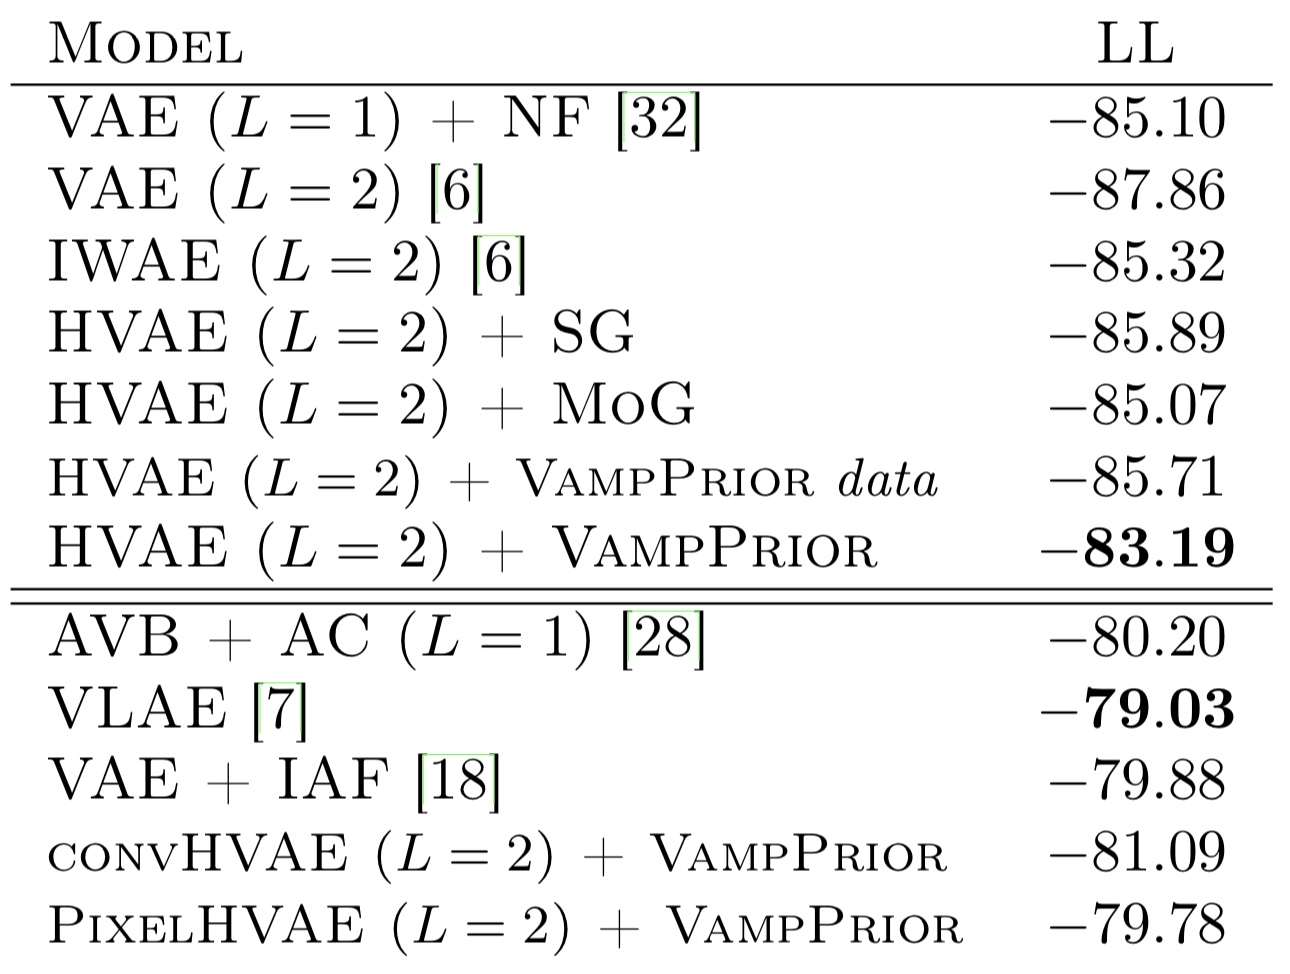
\includegraphics[width=0.9\linewidth]{figs/VampPrior_1.png}
			\end{figure}
		\end{minipage}%
		\begin{minipage}[t]{0.5\columnwidth}
			\begin{figure}[h]
				\centering
				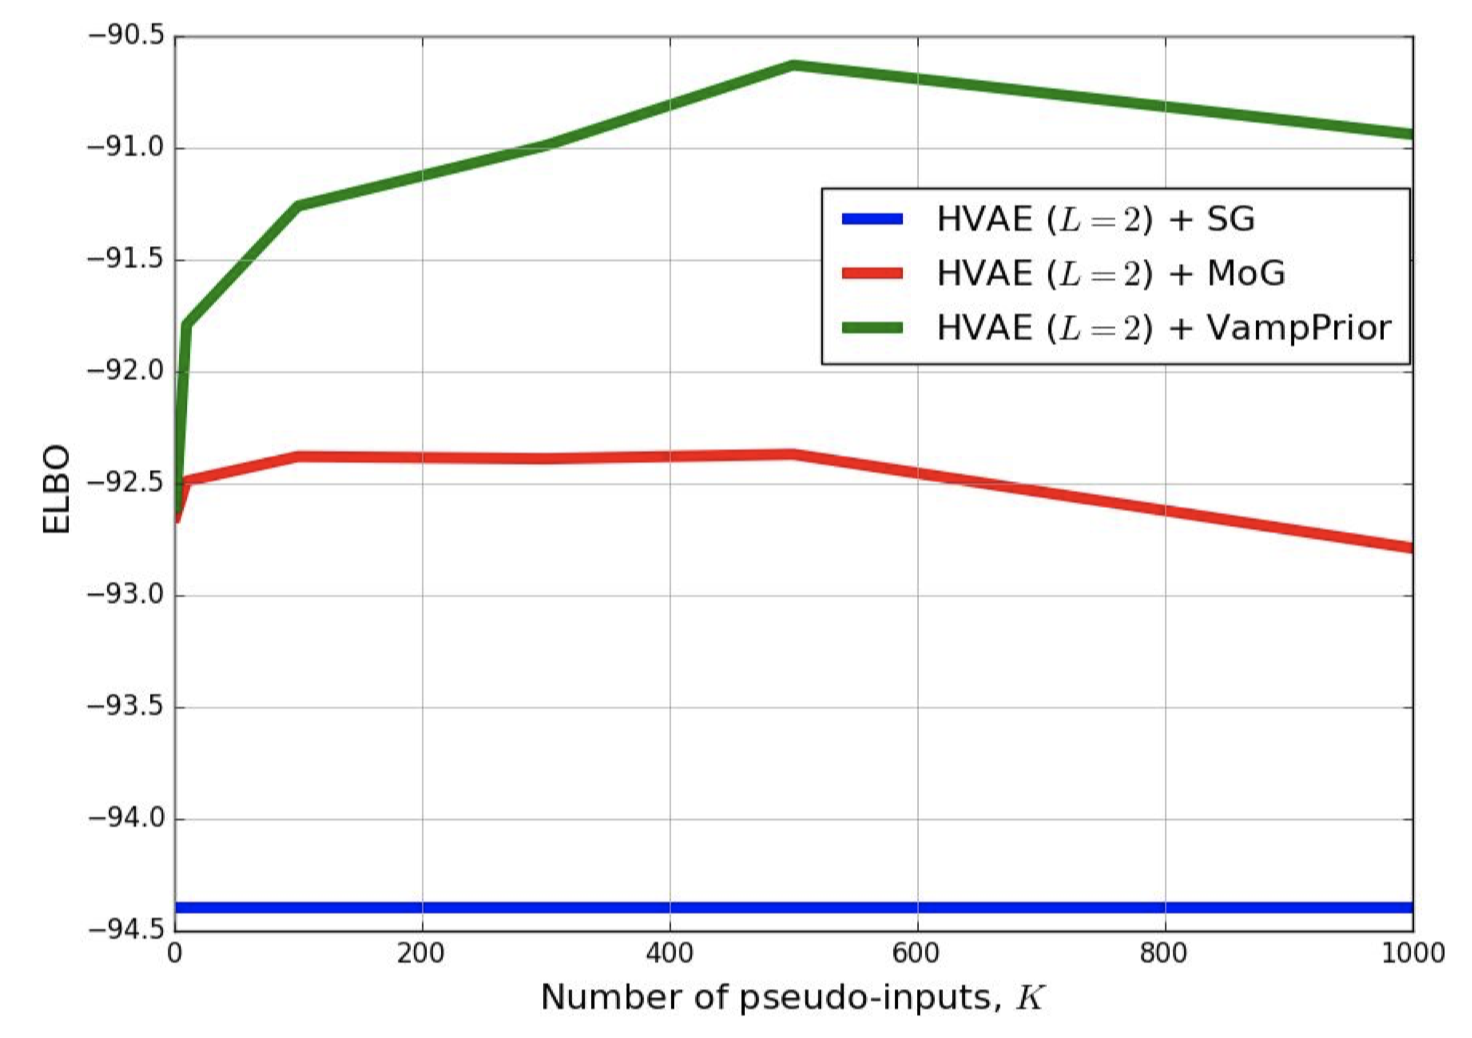
\includegraphics[width=1.\linewidth]{figs/VampPrior_2.png}
			\end{figure}
		\end{minipage}
	\end{block}
	\myfootnotewithlink{https://arxiv.org/abs/1705.07120}{Tomczak J. M., Welling M. VAE with a VampPrior, 2017}
\end{frame}
%=======
\begin{frame}{VampPrior}
	\vspace{0.1cm}
	\textbf{Top row:} generated images by PixelHVAE + VampPrior for chosen pseudo-input in the left top corner. \\
	\vspace{0.1cm}
	\textbf{Bottom row:} pseudo-inputs for different datasets.
	\begin{figure}[h]
		\centering
		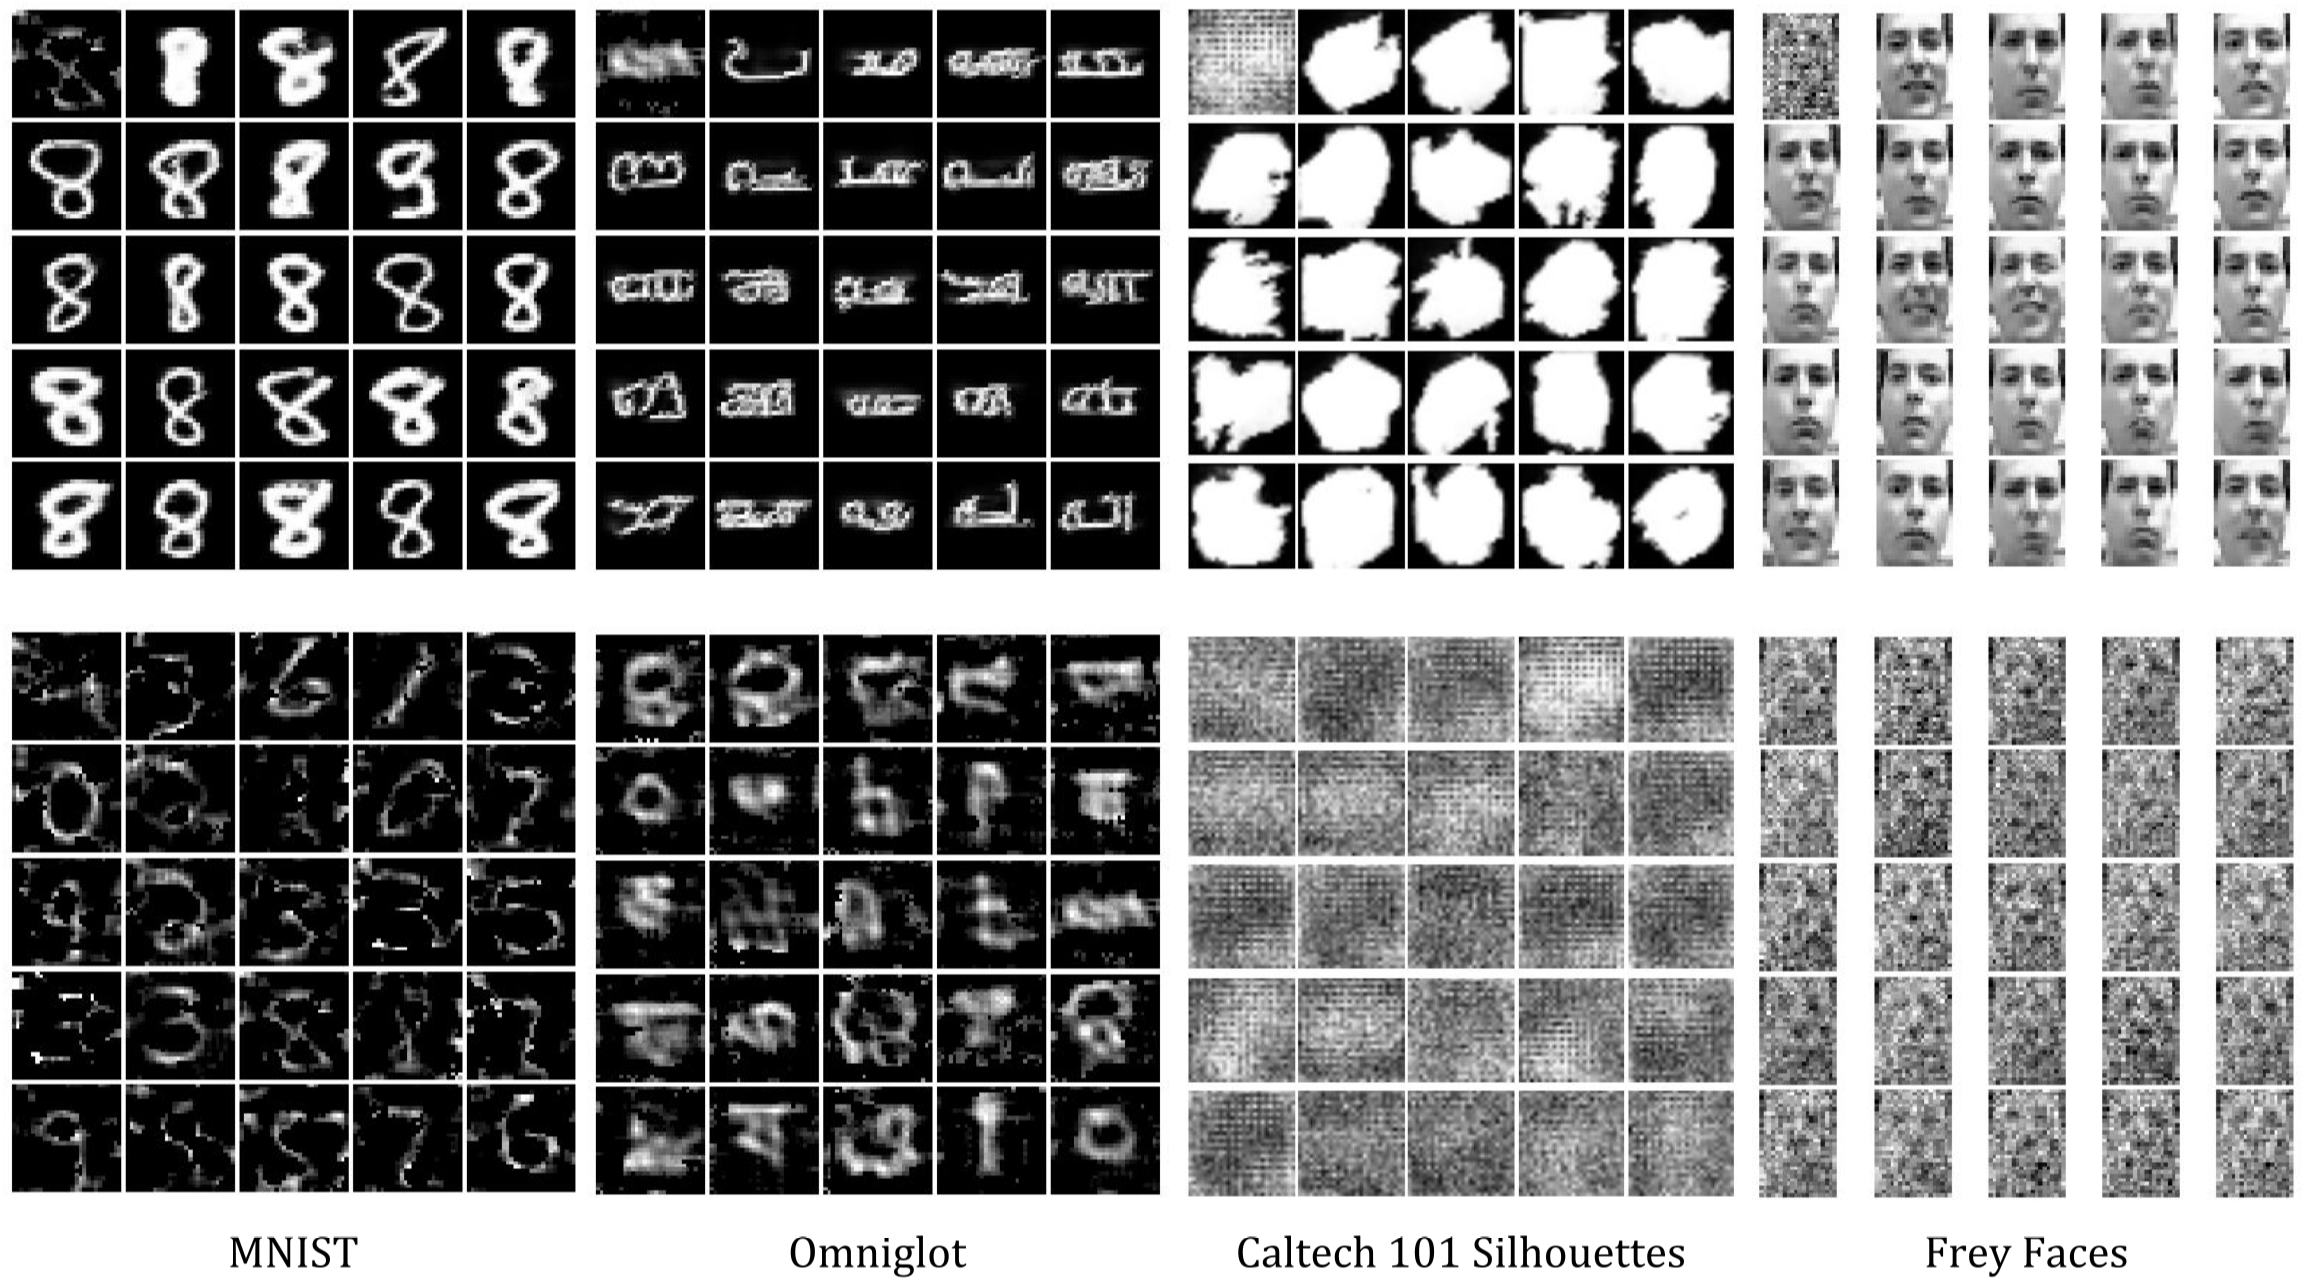
\includegraphics[width=1.0\linewidth]{figs/VampPrior_4.png}
	\end{figure}
	\myfootnotewithlink{https://arxiv.org/abs/1705.07120}{Tomczak J. M., Welling M. VAE with a VampPrior, 2017}
\end{frame}
%=======
\begin{frame}{Flow prior in VAE}
	
	\begin{block}{ELBO revisiting}
		\vspace{-0.4cm}
		\[
		    \frac{1}{n} \sum_{i=1}^n \cL_i(q, \btheta) = \underbrace{\frac{1}{n} \sum_{i=1}^n \mathbb{E}_{q(\bz | \bx_i)} \log p(\bx_i | \bz, \btheta)}_{\text{Reconstruction loss}}
	- \underbrace{\vphantom{ \sum_{i=1}^n} \bbI_q [\bx, \bz]}_{\text{MI}} - \underbrace{\vphantom{ \sum_{i=1}^n} KL(q(\bz) || p(\bz))}_{\text{Marginal KL}}
		\]
	\end{block}
	\vspace{-0.5cm}
	\begin{block}{VampPrior}
		\vspace{-0.5cm}
		\[
			p(\bz | \blambda) = \frac{1}{K} \sum_{k=1}^K q(\bz | \bu_k),
		\]
	where $\bu_1, \dots, \bu_K$ are trainable preudo-inputs.
	\end{block}
	\begin{block}{Autoregressive flow prior}
		\vspace{-0.3cm}
		\[
			\log p(\bz | \blambda) = \log p(\bepsilon) + \log \det \left | \frac{d \bepsilon}{d\bz}\right|
		\]
		\[
			\bz = g(\bepsilon, \blambda) = f^{-1}(\bepsilon, \blambda)
		\]
	\end{block}
	\myfootnotewithlink{https://arxiv.org/abs/1611.02731}{Chen X. et al. Variational Lossy Autoencoder, 2016}
\end{frame}
%=======
\begin{frame}{Flow prior in VAE}
	\begin{block}{Theorem}
	VAE with the AF prior for latent code $\bz$ is equivalent to using the IAF posterior for latent code $\bepsilon$.
	\end{block}
	\begin{block}{Proof}
	\vspace{-0.5cm}
	{\footnotesize
	\begin{align*}
	\mathcal{L}(q, \btheta) &= \mathbb{E}_{q(\bz | \bx)} \left[ \log p(\bx | \bz, \btheta) +  \log p(\bz | \blambda) - \log q(\bz | \bx) \right] \\
	&= \mathbb{E}_{q(\bz | \bx)} \Bigl[ \log p(\bx | \bz, \btheta) + \underbrace{ \Bigl( \log p(f(\bz, \blambda)) + \log \left| \det \frac{\partial f(\bz, \blambda)}{\partial \bz} \right| \Bigr) }_{\text{AF prior}} - \log q(\bz | \bx) \Bigr] \\
	&= \mathbb{E}_{q(\bz | \bx)} \Bigl[ \log p(\bx | \bz, \btheta) +  \log p(f(\bz, \blambda)) - \underbrace{ \Bigl( \log q(\bz | \bx) - \log \left| \det \frac{\partial f(\bz, \blambda)}{\partial \bz} \right| \Bigr) }_{\text{IAF posterior}} \Bigr]
	\end{align*}
	}
	\end{block}
	\vspace{-0.5cm}
	\begin{block}{Flows in VAE}
		\vspace{-0.3cm}
		{\footnotesize
		\[
			\mathcal{L} (\bphi, \btheta) 
			= \mathbb{E}_{q(\bz_0 | \bx, \bphi)} \bigg[\log p(\bx, \bz_K | \btheta) -  \log q(\bz_0 | \bx, \bphi ) +   \log \left| \det \left( \frac{\partial g(\bz_0, \bphi_*)}{\partial \bz_0} \right) \right| \bigg].
		\]
		}
	\end{block}
	\myfootnotewithlink{https://arxiv.org/abs/1611.02731}{Chen X. et al. Variational Lossy Autoencoder, 2016}
\end{frame}
%=======
\begin{frame}{Flow prior in VAE}
	\begin{block}{Autoregressive flow prior}
		{\footnotesize
		\begin{align*}
			\mathcal{L}(q, \btheta) &= \mathbb{E}_{\bz \sim q(\bz | \bx)} \Bigl[ \log p(\bx | \bz, \btheta) + \underbrace{ \Bigl( \log p(f(\bz, \blambda)) + \log \left| \det \frac{\partial f(\bz, \blambda)}{\partial \bz} \right| \Bigr) }_{\text{AF prior}} - \log q(\bz | \bx) \Bigr] \\
			&= \mathbb{E}_{\bz \sim q(\bz | \bx)} \Bigl[ \log p(\bx | \bz, \btheta) +  \log p(f(\bz, \blambda)) - \underbrace{ \Bigl( \log q(\bz | \bx) - \log \left| \det \frac{\partial f(\bz, \blambda)}{\partial \bz} \right| \Bigr) }_{\text{IAF posterior}} \Bigr]
		\end{align*}
		}
	\end{block}
	\begin{itemize}
		\item IAF posterior decoder path: $p(\bx|\bz, \btheta)$, $\bz \sim p(\bz)$.
		\item AF prior decoder path: $p(\bx|\bz, \btheta)$, $\bz = g(\bepsilon, \blambda)$, $\bepsilon \sim p(\bepsilon)$. 
	\end{itemize}
	The AF prior and the IAF posterior have the same computation cost, so using the AF prior makes the model more expressive at no training time cost.

	\myfootnotewithlink{https://arxiv.org/abs/1611.02731}{Chen X. et al. Variational Lossy Autoencoder, 2016}
\end{frame}
%=======
\begin{frame}{VAE limitations}
\begin{itemize}
	\item Poor variational posterior distribution (encoder)
	\[
	q(\bz | \bx, \bphi) = \mathcal{N}(\bz| \bmu_{\bphi}(\bx), \bsigma^2_{\bphi}(\bx)).
	\]
	\item Poor prior distribution
	\[
	p(\bz) = \mathcal{N}(0, \mathbf{I}).
	\]
	\item Poor probabilistic model (decoder)
	\[
	p(\bx | \bz, \btheta) = \mathcal{N}(\bx| \bmu_{\btheta}(\bz), \bsigma^2_{\btheta}(\bz)).
	\]
	\item Loose lower bound
	\[
	\log p(\bx | \btheta) - \mathcal{L}(q, \btheta) = (?).
	\]
\end{itemize}
\end{frame}
%=======
\begin{frame}{Posterior collapse}
	\begin{block}{Representation learning}
		"Identifies and disentangles the underlying causal factors of the data, so that it becomes easier to understand the data, to classify it, or to perform other tasks".
	\end{block}
	\vspace{-0.2cm}
	\[
		p(\bx | \btheta) = \int p(\bx, \bz | \btheta) d \bz = \int p(\bx | \bz, \btheta) p(\bz) d \bz 
	\]
	If the decoder model $p(\bx | \bz, \btheta)$ is powerful enough to model $p(\bx | \btheta)$ the latent variables $\bz$ becomes irrelevant.
	\[
		\mathcal{L}(q, \btheta) = \left[ \mathbb{E}_{q(\bz | \bx)} \log p(\bx | \bz, \btheta) - KL(q(\bz | \bx) || p(\bz)) \right].
	\]
	Early in the training the approximate posterior $q(\bz|\bx)$ carries little information about $\bx$ and the model sets the posterior to the prior to avoid paying any cost $KL(q(\bz|\bx)||p(\bz))$.
\end{frame}
%=======
\begin{frame}{PixelVAE}
	\begin{block}{LVM}
		\vspace{-0.3cm}
		\[
		    p(\bx | \btheta) = \int p(\bx, \bz | \btheta) d \bz = \int p(\bx | \bz, \btheta) p(\bz) d \bz 
		\]
		\vspace{-0.3cm}
	\end{block}
	\begin{itemize}
		\item More powerful $p(\bx | \bz, \btheta)$ leads to more powerful generative model $p(\bx | \btheta)$.
		\item Too powerful $p(\bx | \bz, \btheta)$ could lead to posterior collapse, where variational posterior $q(\bz | \bx)$ will not carry any information about data and close to prior $p(\bz)$.
	\end{itemize}
	How to make the generative model $p(\bx | \bz, \btheta)$ more powerful?
	\begin{block}{Autoregressive decoder}
		\vspace{-0.2cm}
		\[
		    p(\bx | \bz , \btheta) = \prod_{i=1}^n p(x_i | \bx_{1:i - 1}, \bz , \btheta)
		\]
	\end{block}
	
	\myfootnotewithlink{https://arxiv.org/abs/1611.05013}{Gulrajani I. et al. PixelVAE: A Latent Variable Model for Natural Images, 2016}
\end{frame}
%=======
\begin{frame}{PixelVAE}
	\begin{block}{Autoregressive decoder}
		\vspace{-0.3cm}
		\[
		p(\bx | \bz , \btheta) = \prod_{i=1}^n p(x_i | \bx_{1:i - 1}, \bz , \btheta)
		\]
		\vspace{-0.3cm}
	\end{block}
	\begin{itemize}
		\item Global structure is captured by latent variables.
		\item Local statistics are captured by limited receptive field autoregressive model.
	\end{itemize}
	\vspace{-0.1cm}
	\begin{block}{MNIST results}
		\vspace{-0.3cm}
		\begin{figure}
		    \centering
		    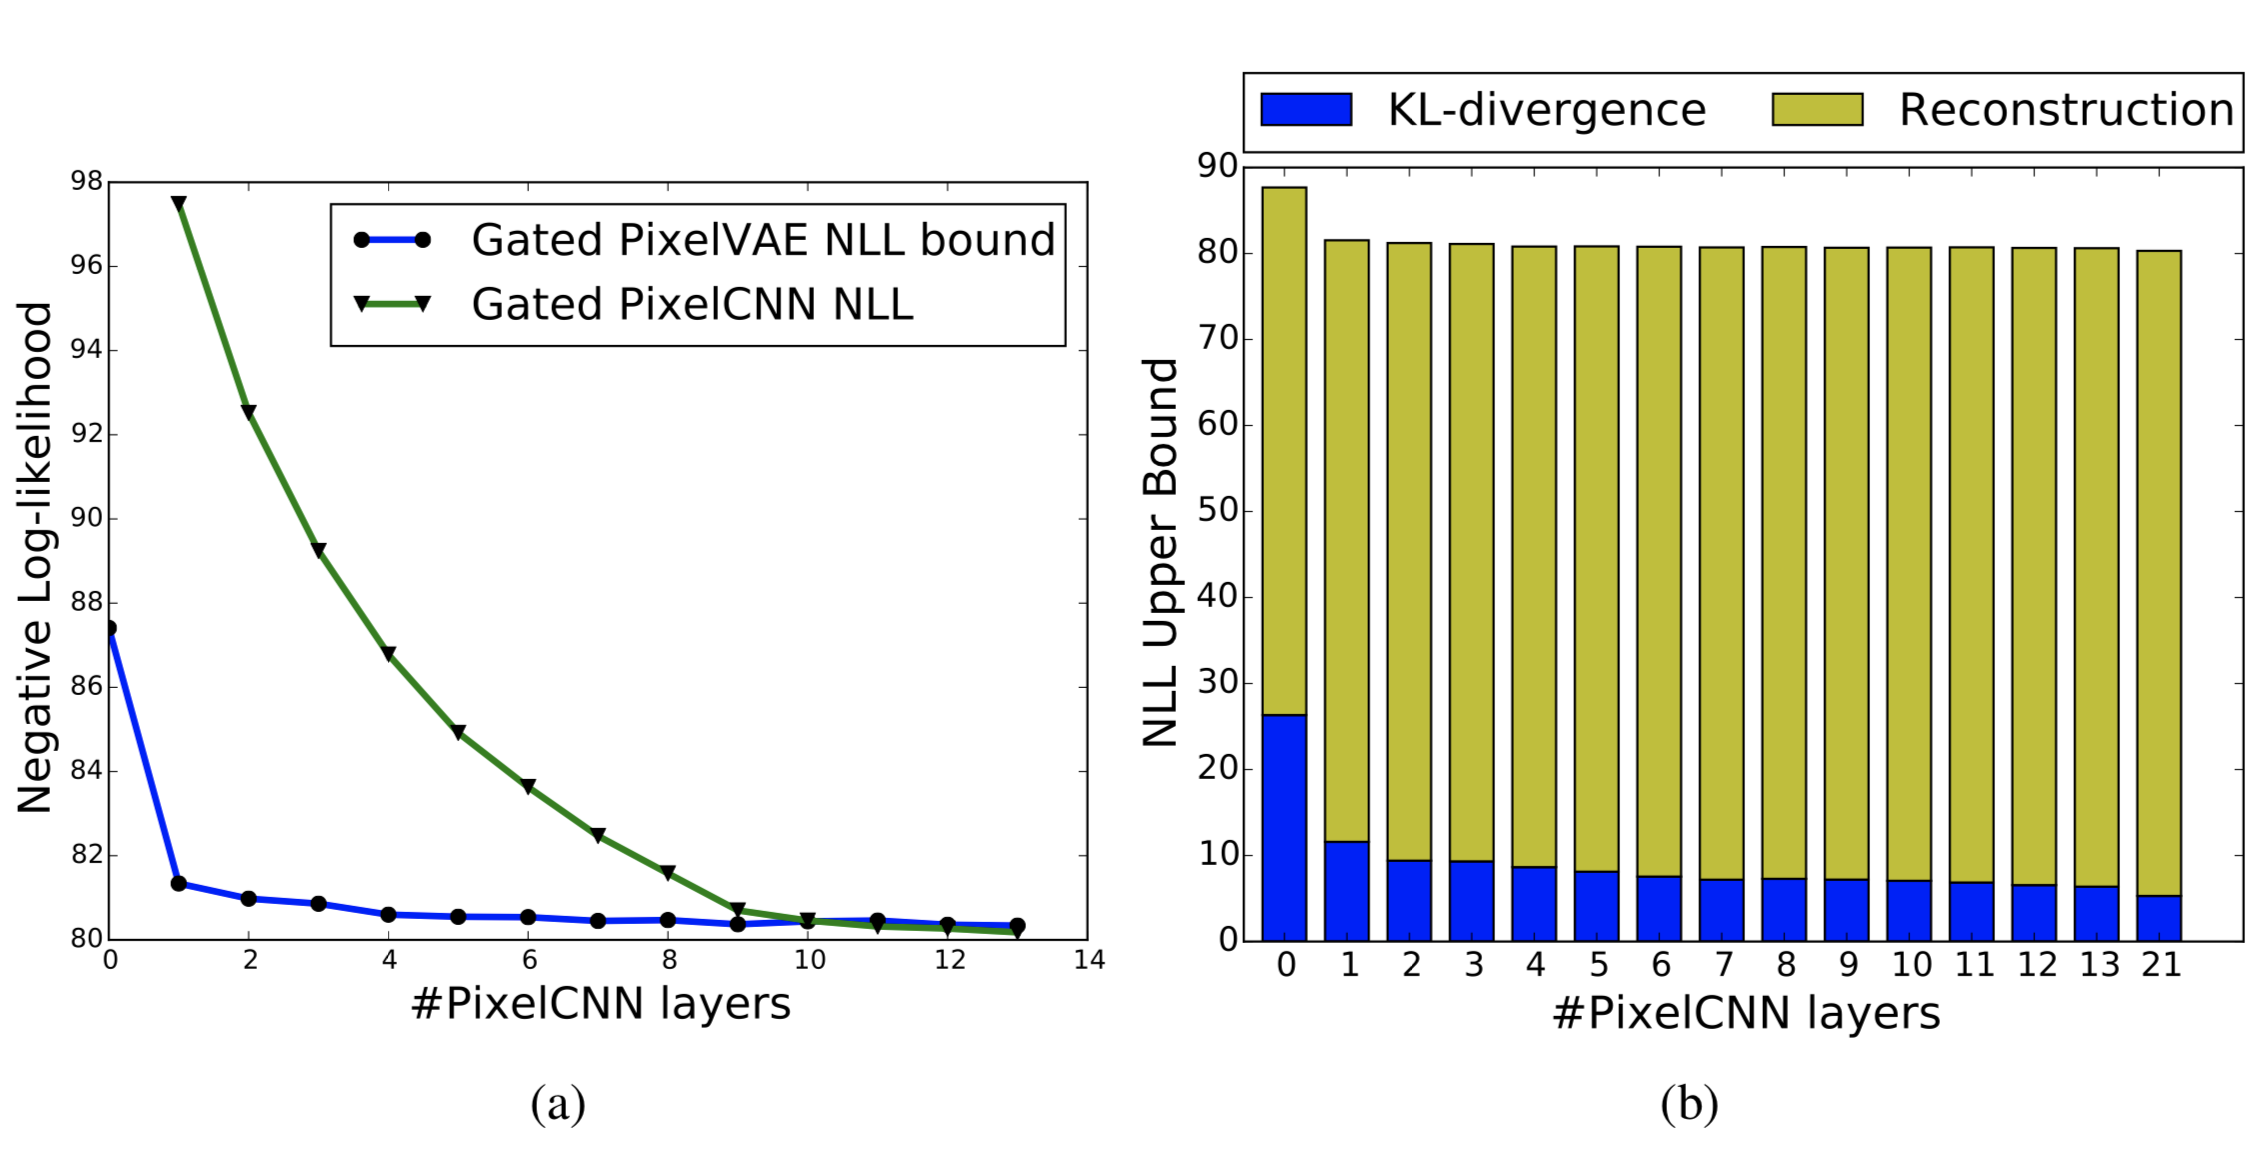
\includegraphics[width=0.75\linewidth]{figs/PixelVAE_2.png}
		\end{figure}
	\end{block}
		
	\myfootnotewithlink{https://arxiv.org/abs/1611.05013}{Gulrajani I. et al. PixelVAE: A Latent Variable Model for Natural Images, 2016}
\end{frame}
%=======
\begin{frame}{PixelVAE}
	\begin{minipage}[t]{0.5\columnwidth}
		MNIST
		\begin{figure}
			\centering
			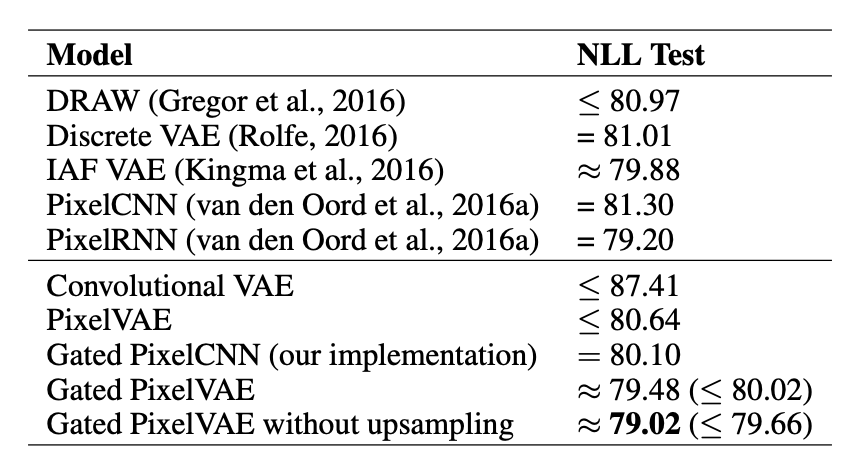
\includegraphics[width=0.9\linewidth]{figs/PixelVAE_5.png}
		\end{figure}
	\end{minipage}%
	\begin{minipage}[t]{0.5\columnwidth}
		ImageNet 64x64
		\begin{figure}
			\centering
			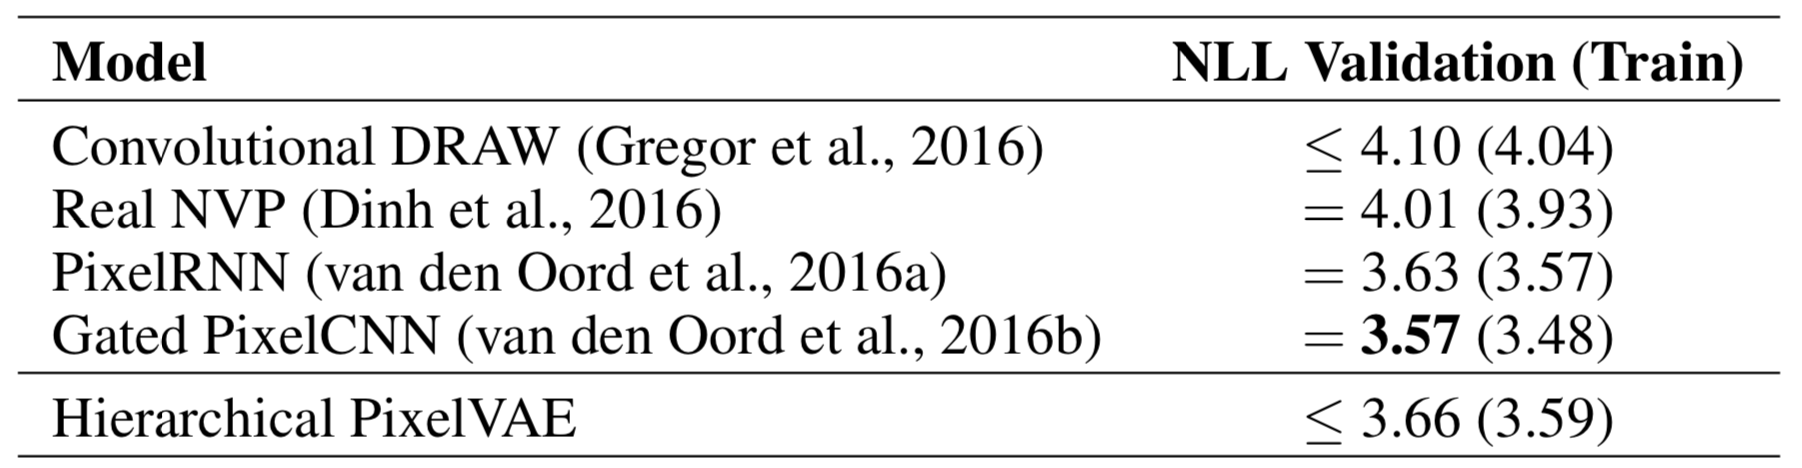
\includegraphics[width=\linewidth]{figs/PixelVAE_4.png}
		\end{figure}
	\end{minipage}
	\begin{figure}
	    \centering
	    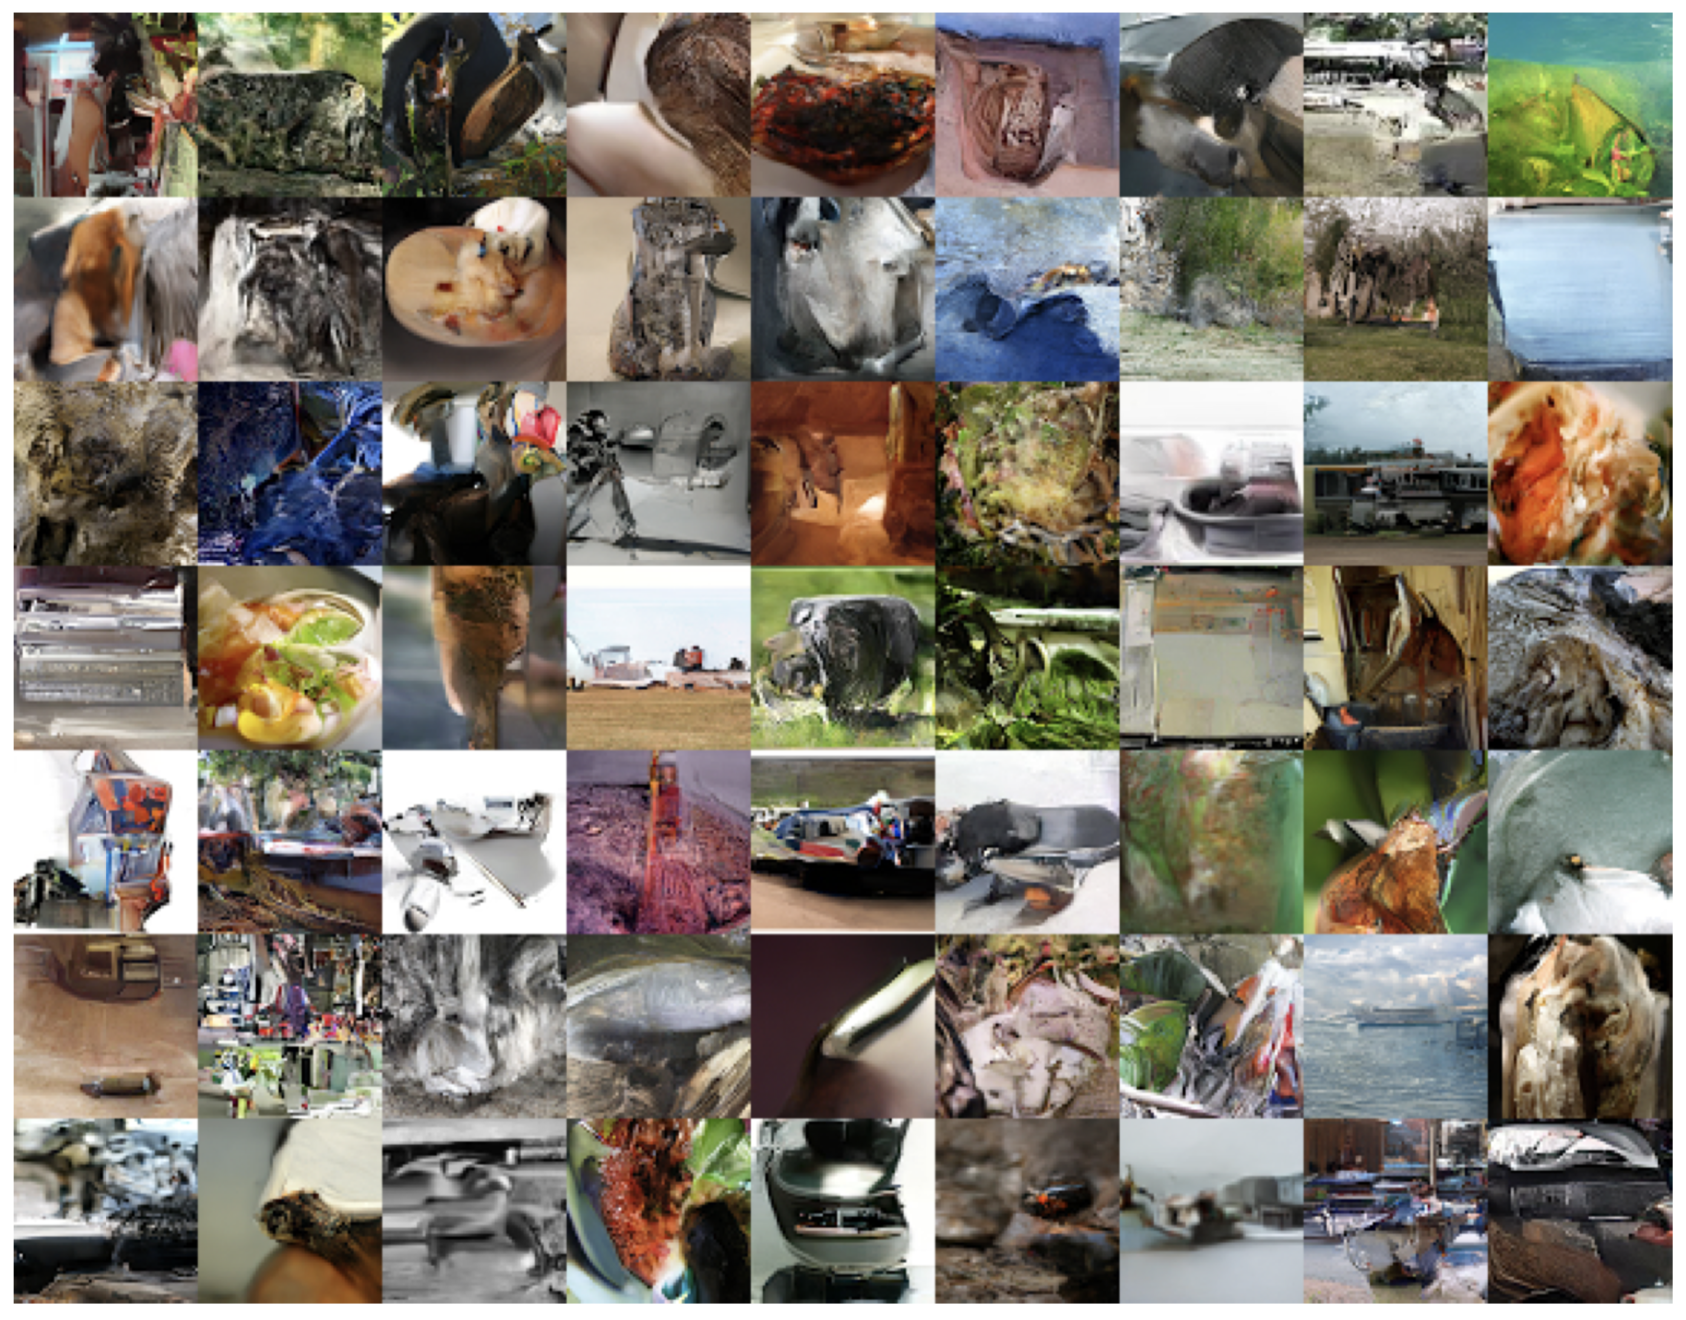
\includegraphics[width=0.5\linewidth]{figs/PixelVAE_3.png}
	\end{figure}
	
	\myfootnotewithlink{https://arxiv.org/abs/1611.05013}{Gulrajani I. et al. PixelVAE: A Latent Variable Model for Natural Images, 2016}
\end{frame}
%=======
\begin{frame}{Decoder weakening}
	\[
		p(\bx | \btheta) = \int p(\bx, \bz | \btheta) d \bz = \int p(\bx | \bz, \btheta) p(\bz) d \bz 
	\]
	\begin{itemize}
		\item Powerful decoder $p(\bx | \bz, \btheta)$ makes the model expressive, but posterior collapse is possible.
		\item PixelVAE model uses the autoregressive PixelCNN model with small number of layers to limit receptive field.
	\end{itemize}
	How to force the model encode information about $\bx$ into $\bz$?
	\[
	    \mathcal{L}(q, \btheta) = \mathbb{E}_{q(\bz | \bx)} \log p(\bx | \bz, \btheta) - \beta \cdot KL (q(\bz | \bx) || p(\bz))
	\]
	What we get if $\beta = 1$ ($\beta = 0$)? \\
	
	\begin{block}{KL annealing}
		\begin{itemize}
		    \item Start training with $\beta = 0$.
		    \item Increase it until $\beta = 1$ during training process.
		\end{itemize}
	\end{block}
	\myfootnotewithlink{https://arxiv.org/abs/1511.06349}{Bowman S. R. et al. Generating Sentences from a Continuous Space, 2015}
\end{frame}
%=======
\begin{frame}{Decoder weakening}
	\begin{block}{Free bits}
	\begin{itemize}
	\item Divide the latent dimensions into the $K$ subsets.
	\item Ensure the use of less than $\lambda$ nats of information per subset $j$.
	\end{itemize}
	\[
	    \hat{\mathcal{L}}(q, \btheta) = \mathbb{E}_{q(\bZ | \bX)} \log p(\bX | \bZ, \btheta) - \sum_{j=1}^K \max(\lambda, KL (q(\bZ_j | \bX) || p(\bZ_j))).
	\]
	Increasing the latent information is advantageous for the reconstruction term. \\
	\vspace{0.2cm}
	This results in $KL (q(\bZ_j | \bX) || p(\bZ_j)) \geq \lambda$ for all $j$, in practice.
	\end{block}
	\myfootnotewithlink{https://arxiv.org/abs/1606.04934}{Kingma D. P. et al. Improving Variational Inference with Inverse Autoregressive Flow, 2016}
\end{frame}
%=======
\begin{frame}{Disentangled representations}
	\begin{block}{Unsupervised representation learning}
	    Learning an interpretable factorised representation of the independent data generative factors of the world without supervision. 
	\end{block}
	\begin{block}{Disentanglement informal definition}
	A disentangled representation can be defined as one where single latent units are sensitive to changes in single generative factors, while being relatively invariant to changes in other factors. 
	\end{block}
	\begin{block}{Example}
	Model trained on a dataset of 3D objects might learn independent latent units sensitive to single independent data generative factors, such as object identity, position, scale, lighting or colour. 
	\end{block}
	\myfootnotewithlink{https://openreview.net/references/pdf?id=Sy2fzU9gl}{Higgins I. et al. beta-VAE: Learning Basic Visual Concepts with a Constrained Variational Framework, 2017}
\end{frame}
%=======
\begin{frame}{Disentanglement learning}
	\begin{block}{Generative process}
	\begin{itemize}
	    \item $p(\bx | \bv, \bw) = \text{Sim}(\bv, \bw)$~-- true world simulator;
	    \item $\bv$~-- conditionally independent factors: $p(\bv | \bx) = \prod_{j=1}^d p(v_j | \bx)$;
	    \item $\bw$~-- conditionally dependent factors. 
	\end{itemize}
	\end{block}
	\begin{block}{Goal}
	Construct an unsupervised deep generative model
	\[
	    p(\bx | \bz) \approx p(\bx | \bv, \bw).
	\]
	\vspace{-0.5cm}
	\begin{itemize}
	    \item Ensure that the inferred latent factors $q(\bz|\bx)$ capture the factors $\bv$ in a disentangled manner. 
	    \item The conditionally dependent factors $\bw$ can remain entangled in a separate subset of $\bz$ that is not used for representing $\bv$. 
	\end{itemize}
	\end{block}
	\myfootnotewithlink{https://openreview.net/references/pdf?id=Sy2fzU9gl}{Higgins I. et al. beta-VAE: Learning Basic Visual Concepts with a Constrained Variational Framework, 2017}
\end{frame}
%=======
\begin{frame}{$\beta$-VAE}
	\begin{block}{ELBO objective}
	\vspace{-0.2cm}
	\[
	    \mathcal{L}(q, \btheta, \beta) = \mathbb{E}_{q(\bz | \bx)} \log p(\bx | \bz, \btheta) - \beta \cdot KL (q(\bz | \bx) || p(\bz)).
	\]
	\vspace{-0.5cm}
	\end{block}
	What do we get at $\beta = 1$? \\
	\begin{block}{Constrained optimization}
		\vspace{-0.5cm}
		\[
			\max_{q, \btheta} \mathbb{E}_{q(\bz | \bx)} \log p(\bx | \bz, \btheta), \quad \text{subject to } KL (q(\bz | \bx) || p(\bz)) < \epsilon.
		\]
		\vspace{-0.5cm}
	\end{block}
	\begin{block}{Hypothesis}
	We are able to learn disentangled representations of the independent factors $\bv$ by setting a stronger constraint with $\beta > 1$.
	\end{block}
	\textbf{Note:} It leads to poorer reconstructions and a loss of high frequency details. 
	\myfootnotewithlink{https://openreview.net/references/pdf?id=Sy2fzU9gl}{Higgins I. et al. beta-VAE: Learning Basic Visual Concepts with a Constrained Variational Framework, 2017}
\end{frame}
%=======
\begin{frame}{$\beta$-VAE}
	\begin{figure}
	    \centering
	    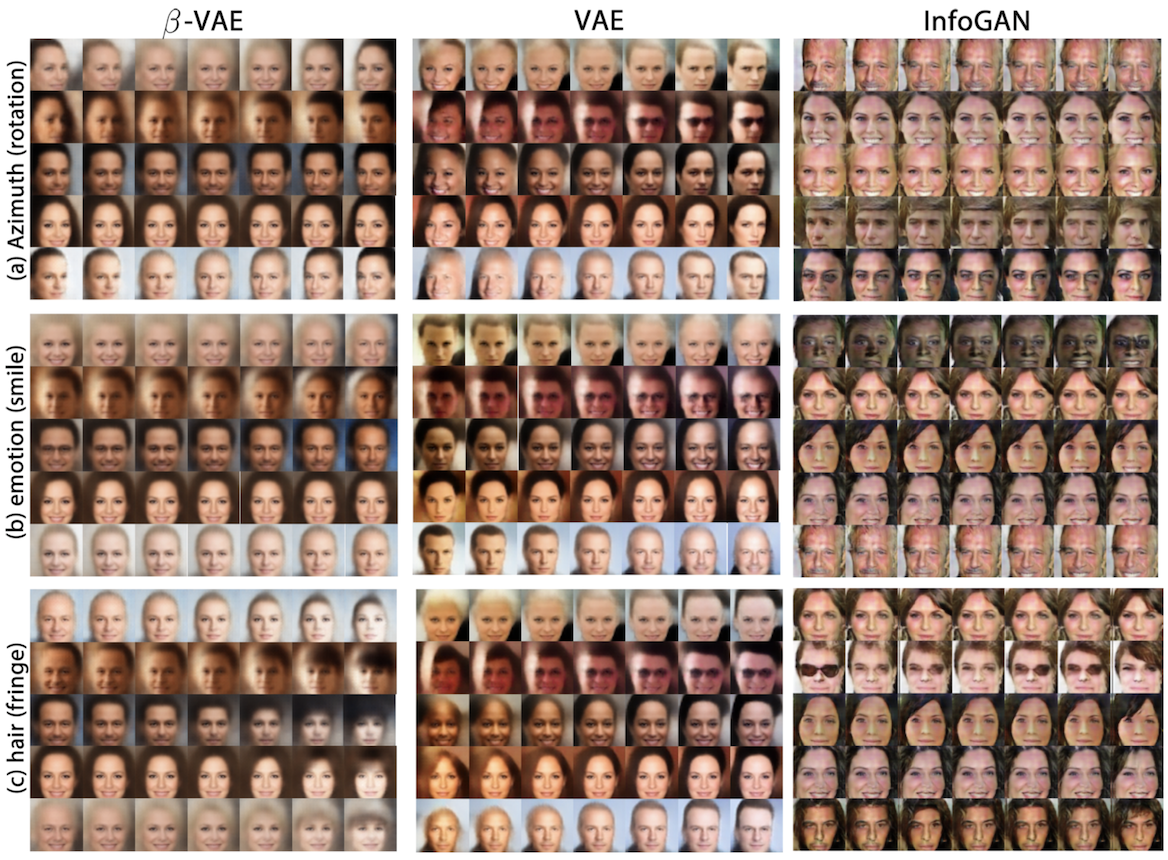
\includegraphics[width=0.95\linewidth]{figs/betaVAE_1.png}
	\end{figure}

	\myfootnotewithlink{https://openreview.net/references/pdf?id=Sy2fzU9gl}{Higgins I. et al. beta-VAE: Learning Basic Visual Concepts with a Constrained Variational Framework, 2017}
\end{frame}
%=======
\begin{frame}{$\beta$-VAE}
	\begin{figure}
	    \centering
	    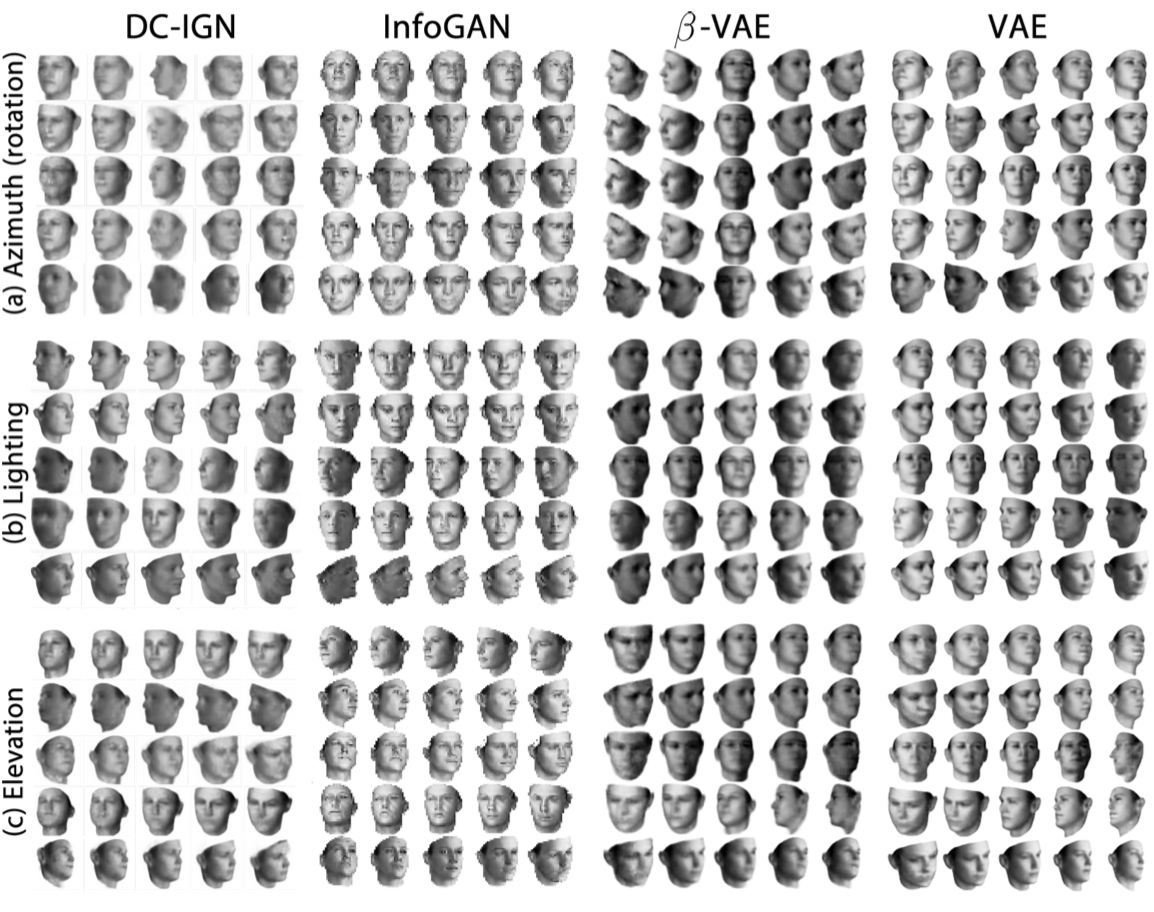
\includegraphics[width=0.9\linewidth]{figs/betaVAE_3.png}
	\end{figure}

	\myfootnotewithlink{https://openreview.net/references/pdf?id=Sy2fzU9gl}{Higgins I. et al. beta-VAE: Learning Basic Visual Concepts with a Constrained Variational Framework, 2017}
\end{frame}
%=======
\begin{frame}{$\beta$-VAE}
		\begin{figure}[h]
			\centering
			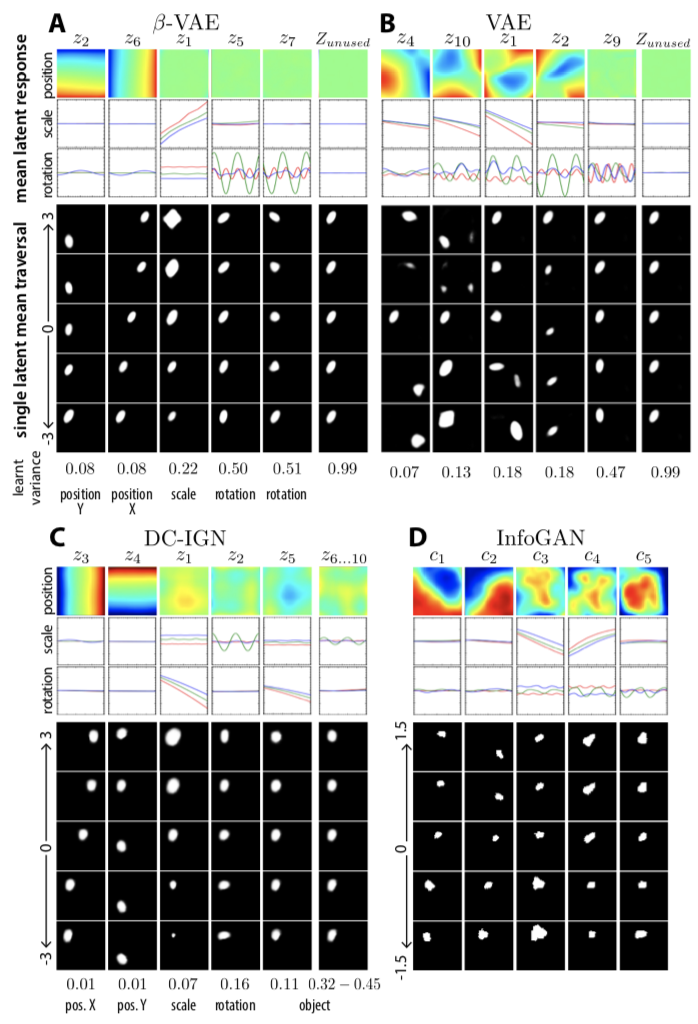
\includegraphics[width=.9\linewidth]{figs/betaVAE_5.png}
		\end{figure}

	\myfootnotewithlink{https://openreview.net/references/pdf?id=Sy2fzU9gl}{Higgins I. et al. beta-VAE: Learning Basic Visual Concepts with a Constrained Variational Framework, 2017}
\end{frame}
%=======
\begin{frame}{$\beta$-VAE}
	\begin{block}{ELBO}
		\vspace{-0.2cm}
		\[
		\mathcal{L}(q, \btheta, \beta) = \mathbb{E}_{q(\bz | \bx)} \log p(\bx | \bz, \btheta) - \beta \cdot KL(q(\bz | \bx) || p(\bz)).
		\]
		\vspace{-0.4cm}
	\end{block}
	\begin{block}{ELBO surgery}
		\vspace{-0.3cm}
		{\footnotesize
			\[
			\frac{1}{n} \sum_{i=1}^n \cL_i(q, \btheta, \beta) = \underbrace{\frac{1}{n} \sum_{i=1}^n \mathbb{E}_{q(\bz | \bx_i)} \log p(\bx_i | \bz, \btheta)}_{\text{Reconstruction loss}} - \beta \cdot \underbrace{\bbI_{q} [\bx, \bz]\vphantom{\sum_{i=1}}}_{\text{MI}} - \beta \cdot \underbrace{KL(q(\bz) || p(\bz))\vphantom{\sum_{i=1}}}_{\text{Marginal KL}}
			\]}
	\end{block}
	\begin{block}{Minimization of MI}
	\begin{itemize}
		\item It is not necessary and not desirable for disentanglement. 
		\item It hurts reconstruction.
	\end{itemize}
	\end{block}
	\myfootnotewithlink{https://arxiv.org/abs/1804.03599}{Burgess C. P. et al. Understanding disentangling in $\beta$-VAE, 2018}
\end{frame}
%=======
\begin{frame}{DIP-VAE}
	\begin{block}{Disentangled aggregated variational posterior}
		\vspace{-0.3cm}
		\[
		q(\bz) = \frac{1}{n} \sum_{i=1}^n q(\bz | \bx) = \prod_{j=1}^d q(z_j)
		\]
		\vspace{-0.3cm}
	\end{block}
	\begin{block}{DIP-VAE Objective}
		\vspace{-0.3cm}
		{\footnotesize
			\begin{multline*}
			\cL_{\text{DIP}}(q, \btheta) = \frac{1}{n} \sum_{i=1}^n \cL_i(q, \btheta) -\lambda \cdot KL(q(\bz) || p(\bz)) = \\
			= \frac{1}{n} \sum_{i=1}^n\left[ \bbE_{q(\bz | \bx_i)} \log p(\bx_i | \bz, \btheta) - KL(q(\bz | \bx_i) || p(\bz)) \right] -\lambda \cdot KL(q(\bz) || p(\bz)) = \\
			= \underbrace{ \frac{1}{n} \sum_{i=1}^n \left[\bbE_{q(\bz | \bx_i)} \log p(\bx_i | \bz, \btheta)\right]}_{\text{Reconstruction loss}} - \underbrace{\vphantom{\sum_{i=1}^n} \bbI_{q} [\bx, \bz]}_{\text{MI}} - (1 + \lambda) \cdot \underbrace{\vphantom{\sum_{i=1}^n} KL(q(\bz) || p(\bz))}_{\text{Marginal KL}}
			\end{multline*}
		}
		\vspace{-0.3cm}
	\end{block}

	\myfootnotewithlink{https://arxiv.org/abs/1711.00848}{Kumar A., Sattigeri P., Balakrishnan A. Variational Inference of Disentangled Latent Concepts from Unlabeled Observations, 2017}
\end{frame}
%=======
\begin{frame}{DIP-VAE}
		\vspace{-0.2cm}
		\[
			\cL_{\text{DIP}}(q, \btheta) = \frac{1}{n} \sum_{i=1}^n \cL_i(q, \btheta) -\lambda \cdot \underbrace{KL(q(\bz) || p(\bz))}_{\text{intractable}}
		\]
	Let match the moments of $q(\bz)$ and $p(\bz)$:
	\[
	\text{cov}_{q(\bz)}(\bz) = \bbE_{q(\bz)} \left[ (\bz - \bbE_{q(\bz)}(\bz)) (\bz - \bbE_{q(\bz)}(\bz))^T \right]
	\]
	DIP-VAE regularizes $\text{cov}_{q(\bz)}(\bz) $ to be close to the identity matrix. 
	\begin{block}{Objective}
		\vspace{-0.5cm}
		\begin{multline*}
		\max_{q, \btheta} \Bigl[\frac{1}{n} \sum_{i=1}^n \cL_i(q, \btheta) - \\ - \lambda_1 \sum_{i \neq j} \left[\text{cov}_{q(\bz)} (\bz) \right]^2_{ij} - \lambda_2 \sum_{i} \left( \left[ \text{cov}_{q(\bz)} (\bz) \right]_{ii} - 1 \right)^2 \Bigr]
		\end{multline*}
		\vspace{-0.5cm}
	\end{block}

	\myfootnotewithlink{https://arxiv.org/abs/1711.00848}{Kumar A., Sattigeri P., Balakrishnan A. Variational Inference of Disentangled Latent Concepts from Unlabeled Observations, 2017}
\end{frame}
%=======
\begin{frame}{DIP-VAE}
	\begin{figure}
		\centering
		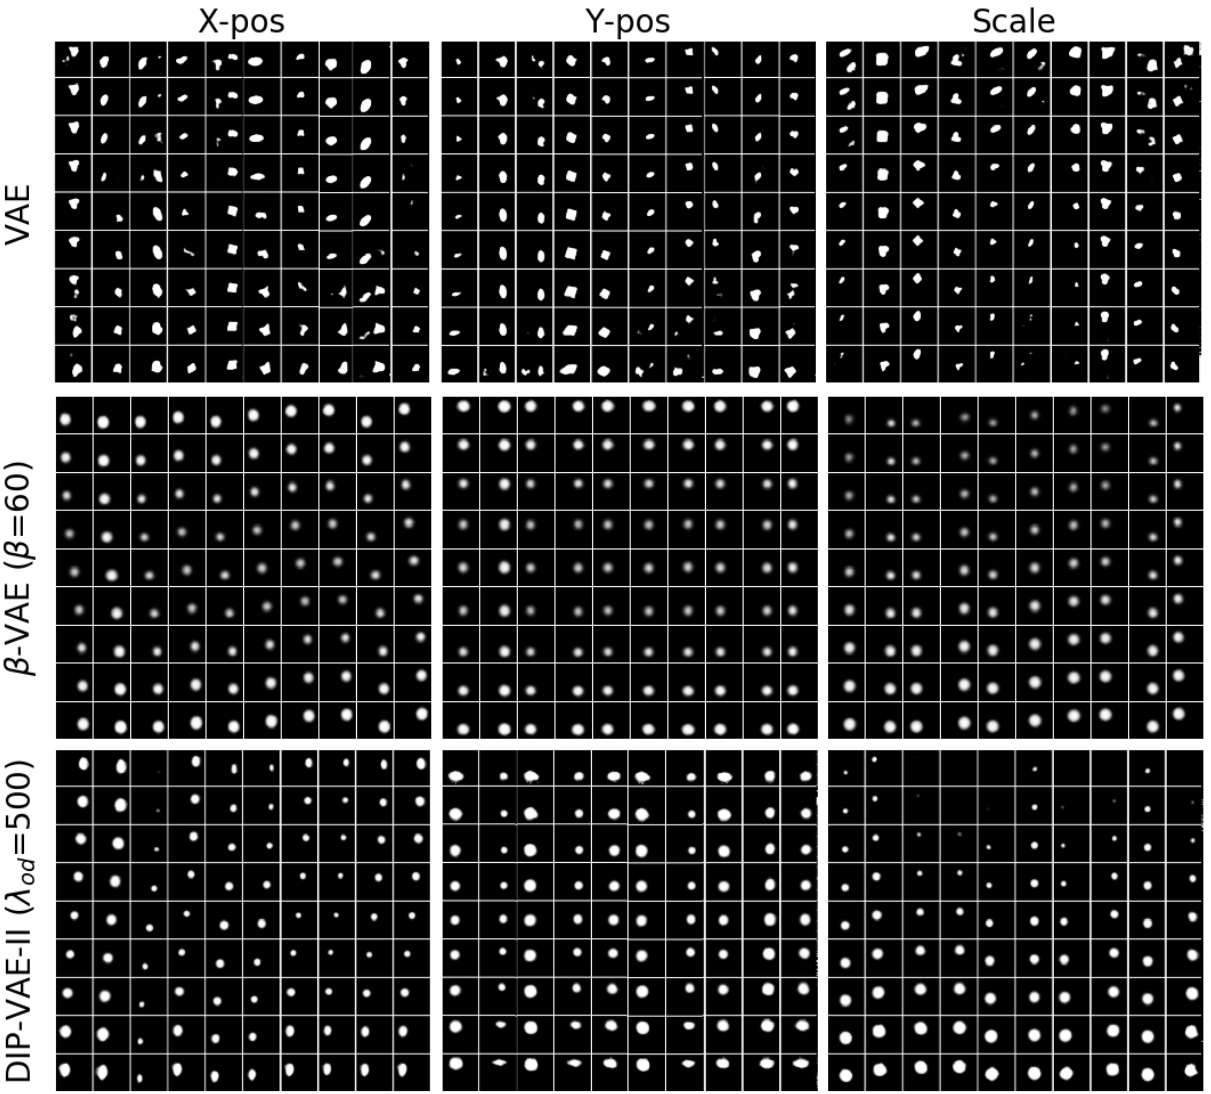
\includegraphics[width=0.75\linewidth]{figs/dip-vae_1}
	\end{figure}

	\myfootnotewithlink{https://arxiv.org/abs/1711.00848}{Kumar A., Sattigeri P., Balakrishnan A. Variational Inference of Disentangled Latent Concepts from Unlabeled Observations, 2017}
\end{frame}
%=======
\begin{frame}{DIP-VAE}
	\begin{figure}
		\centering
		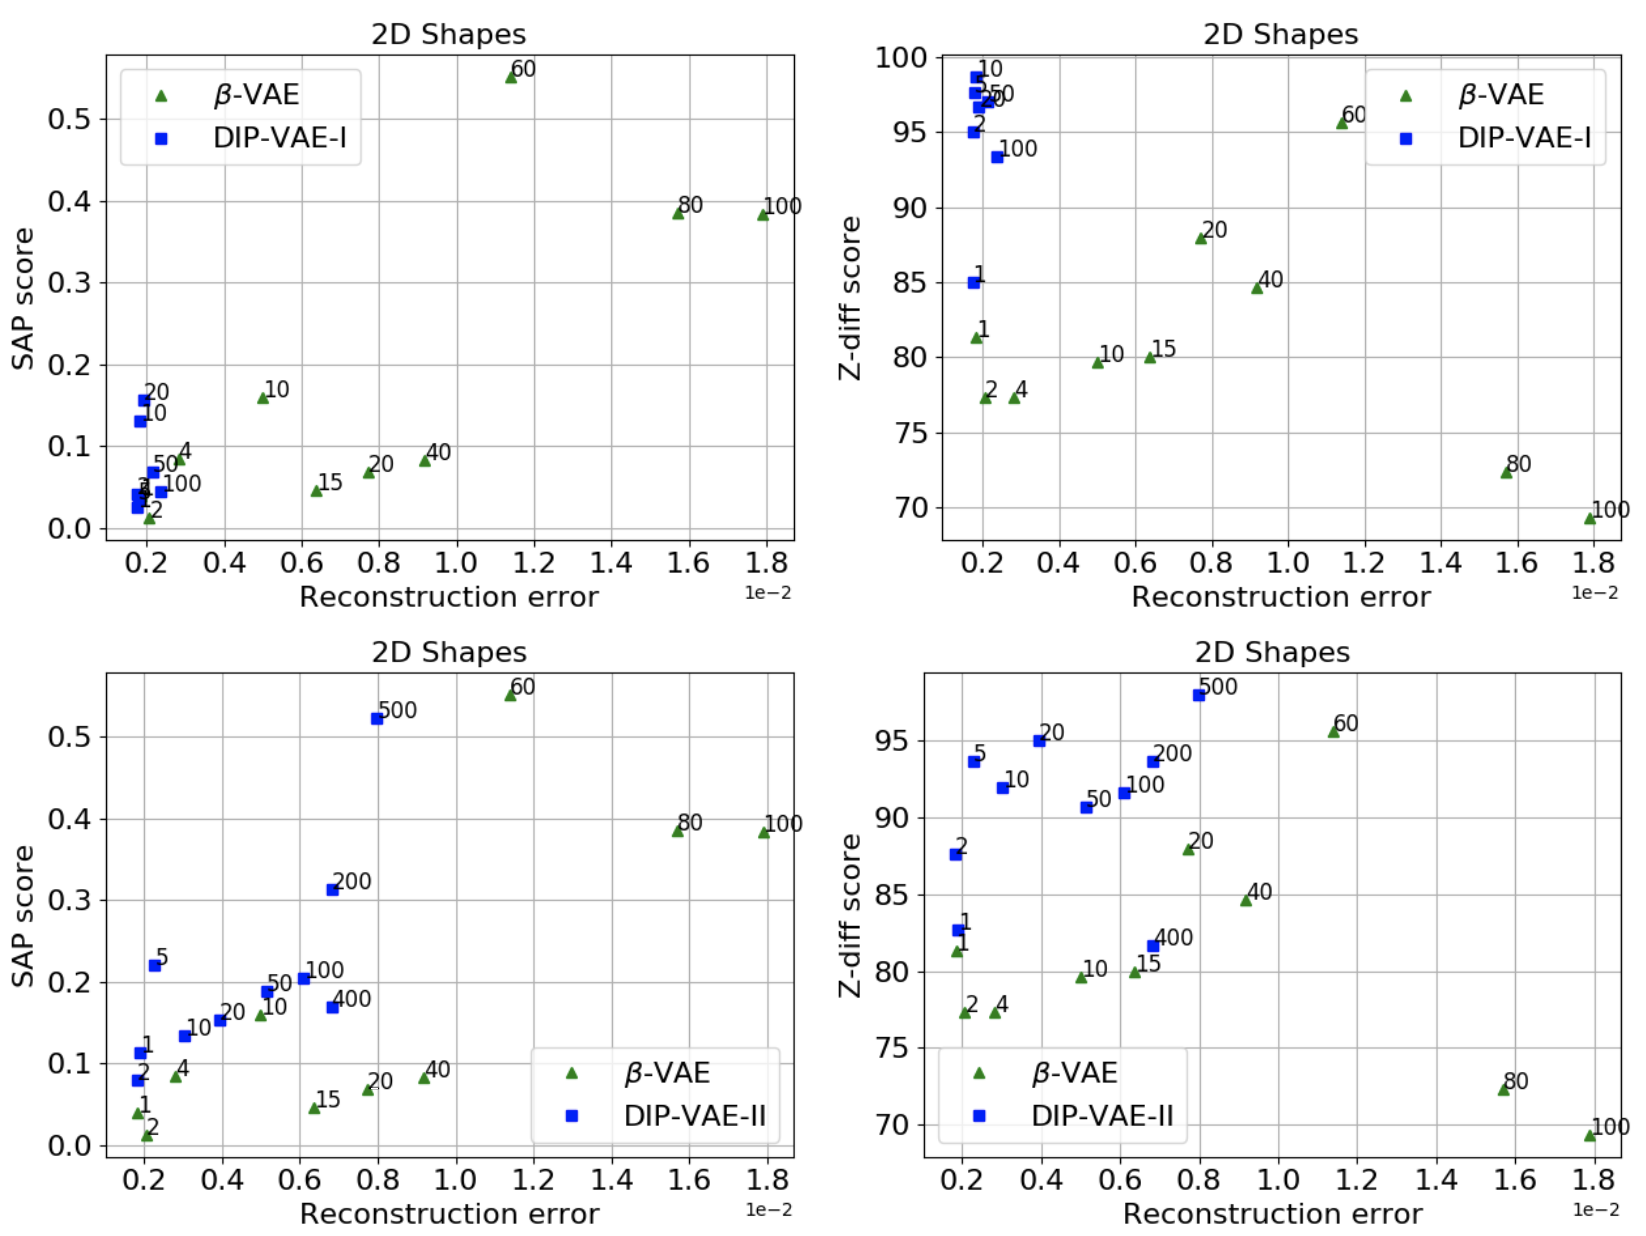
\includegraphics[width=0.9\linewidth]{figs/dip-vae_2}
	\end{figure}

	\myfootnotewithlink{https://arxiv.org/abs/1711.00848}{Kumar A., Sattigeri P., Balakrishnan A. Variational Inference of Disentangled Latent Concepts from Unlabeled Observations, 2017}
\end{frame}
%=======
\begin{frame}{FactorVAE}
	\begin{block}{Disentangled aggregated variational posterior}
		\vspace{-0.3cm}
		\[
		q(\bz) = \bbE_{\pi(\bx)} q(\bz | \bx) = \int q(\bz | \bx) \pi(\bx) d\bx = \prod_{j=1}^d q(z_j)
		\]
		\vspace{-0.3cm}
	\end{block}
	\begin{block}{Total correlation regularizer}
		\vspace{-0.3cm}
		\[
		\min KL(q(\bz) || \prod_{j=1}^d q(z_j))
		\]
		\vspace{-0.3cm}
	\end{block}
	\begin{block}{FactorVAE objective}
		\vspace{-0.3cm}
		\[
		\min_{\btheta, \bphi} \text{ELBO}(\btheta, \bphi) - \gamma \cdot KL(q(\bz) || \prod_{j=1}^d q(z_j))
		\]
		\vspace{-0.3cm}
	\end{block}
	\begin{itemize}
		\item The last term is intractable.
		\item FactorVAE uses density ratio trick for estimation. 
	\end{itemize}

	\myfootnotewithlink{https://arxiv.org/abs/1802.05983}{Kim H., Mnih A. Disentangling by Factorising, 2018}
\end{frame}
%=======
\begin{frame}{FactorVAE}
	Consider two distributions $q_1(\bx)$, $q_2(\bx)$ and probilistic model
	\[
		p(\bx | y) = \begin{cases}
			q_1(\bx), \text{ if } y = 1, \\
			q_2(\bx), \text{ if } y = 0,
		\end{cases}
		\quad 
		y \sim \text{Bern}(0.5).
	\]
	\begin{block}{Density ratio trick}
		\vspace{-0.5cm}
		\begin{multline*}
			\frac{q_1(\bx)}{q_2(\bx)} = \frac{p(\bx | y = 1)}{p(\bx | y = 0)} = \frac{p(y = 1 | \bx) p(\bx)}{p(y=1)} \bigg/ \frac{p(y = 0 | \bx) p(\bx)}{p(y=0)} = \\
			= \frac{p(y = 1 | \bx)}{p(y = 0 | \bx)} = \frac{p(y = 1 | \bx)}{1 - p(y = 1 | \bx)} = \frac{D(\bx)}{1 - D(\bx)}
		\end{multline*}
	Here $D(\bx)$ could be treated as a discriminator a model the output of which is a probability that $\bx$ is a sample
	from $q_1(\bx)$ rather than from $q_2(\bx)$.
	\end{block}

	\myfootnotewithlink{https://arxiv.org/abs/1802.05983}{Kim H., Mnih A. Disentangling by Factorising, 2018}
\end{frame}
%=======
\begin{frame}{FactorVAE}
	
	\begin{block}{FactorVAE objective}
		\vspace{-0.3cm}
		\[
		\min_{\btheta, \bphi} \text{ELBO}(\btheta, \bphi) - \gamma \cdot KL(q(\bz) || \prod_{j=1}^d q(z_j))
		\]
		\vspace{-0.3cm}
	\end{block}
	
	\begin{block}{Total correlation regularizer}
		\vspace{-0.7cm}
		\begin{multline*}
		KL(q(\bz) || \prod_{j=1}^d q(z_j)) = KL(q(\bz) || \bar{q}(\bz)) = \\ =\bbE_{q(\bz)} \log \frac{q(\bz)}{\bar{q}(\bz)} \approx \bbE_{q(\bz)} \log \frac{D(\bz)}{1 - D(\bz)}
		\end{multline*}
		\vspace{-0.3cm}
	\end{block}
	VAE and GAN are trained simultaneously.

	\myfootnotewithlink{https://arxiv.org/abs/1802.05983}{Kim H., Mnih A. Disentangling by Factorising, 2018}
\end{frame}
%=======
\begin{frame}{FactorVAE}
	
	\begin{minipage}[t]{0.5\columnwidth}
		\begin{figure}
			\centering
			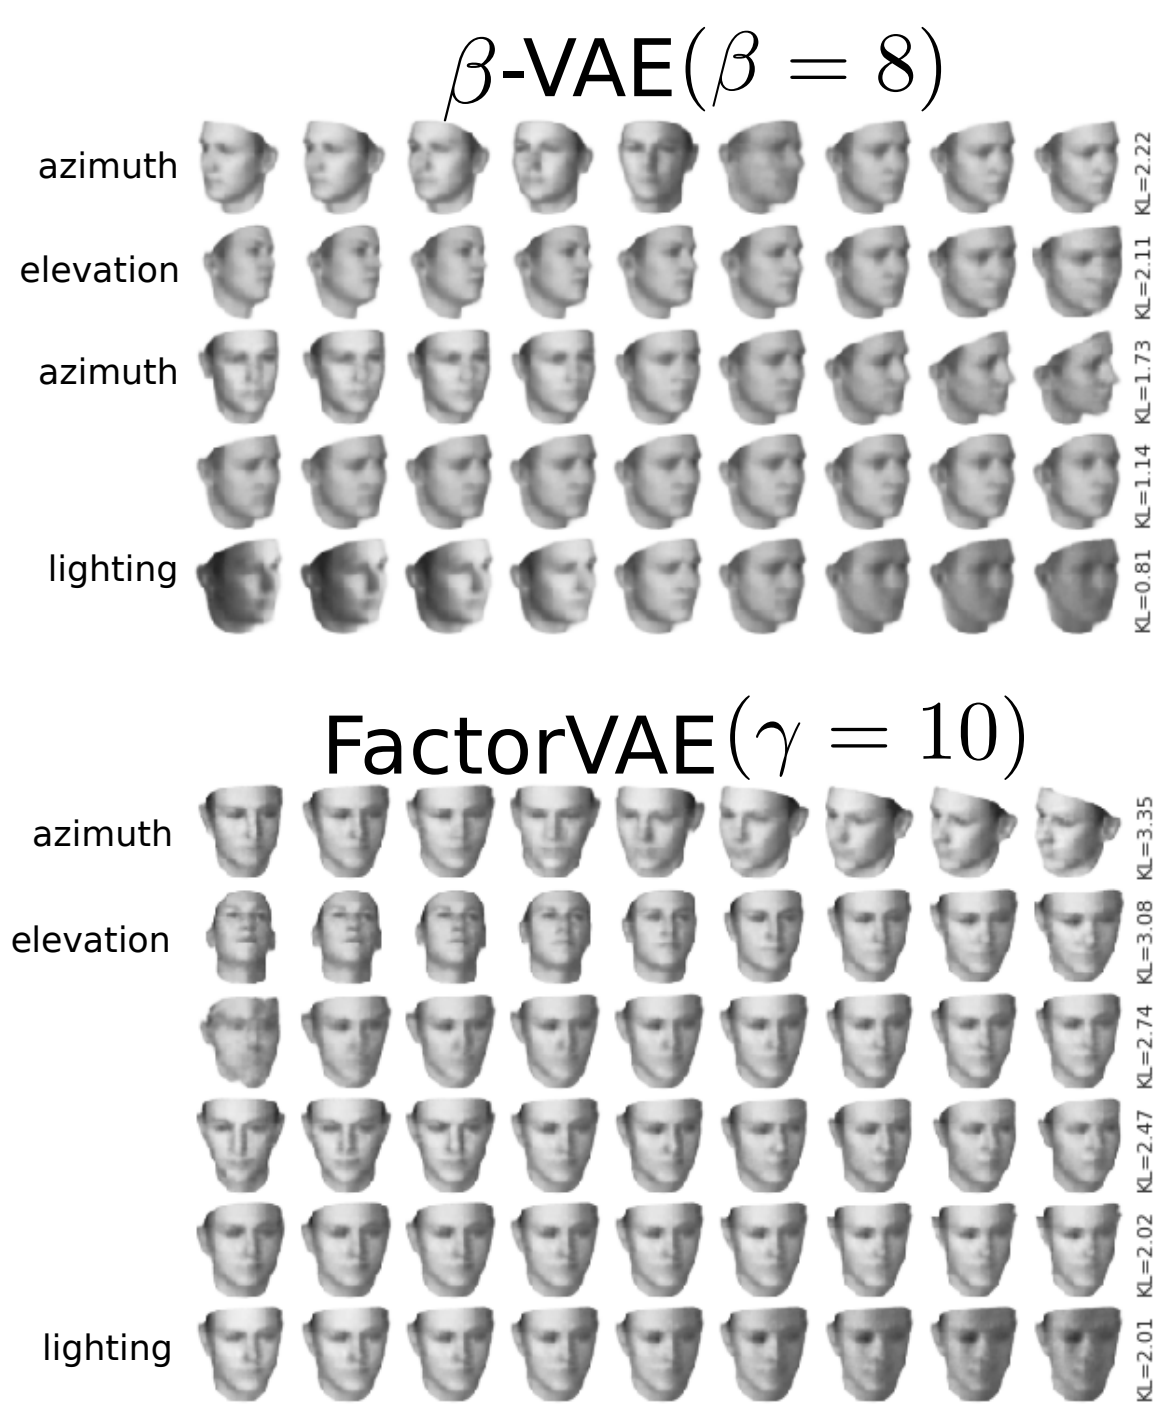
\includegraphics[width=\linewidth]{figs/factorvae_1}
		\end{figure}
	\end{minipage}%
	\begin{minipage}[t]{0.5\columnwidth}
		\vspace{1.7cm}
		\begin{figure}[h]
			\centering
			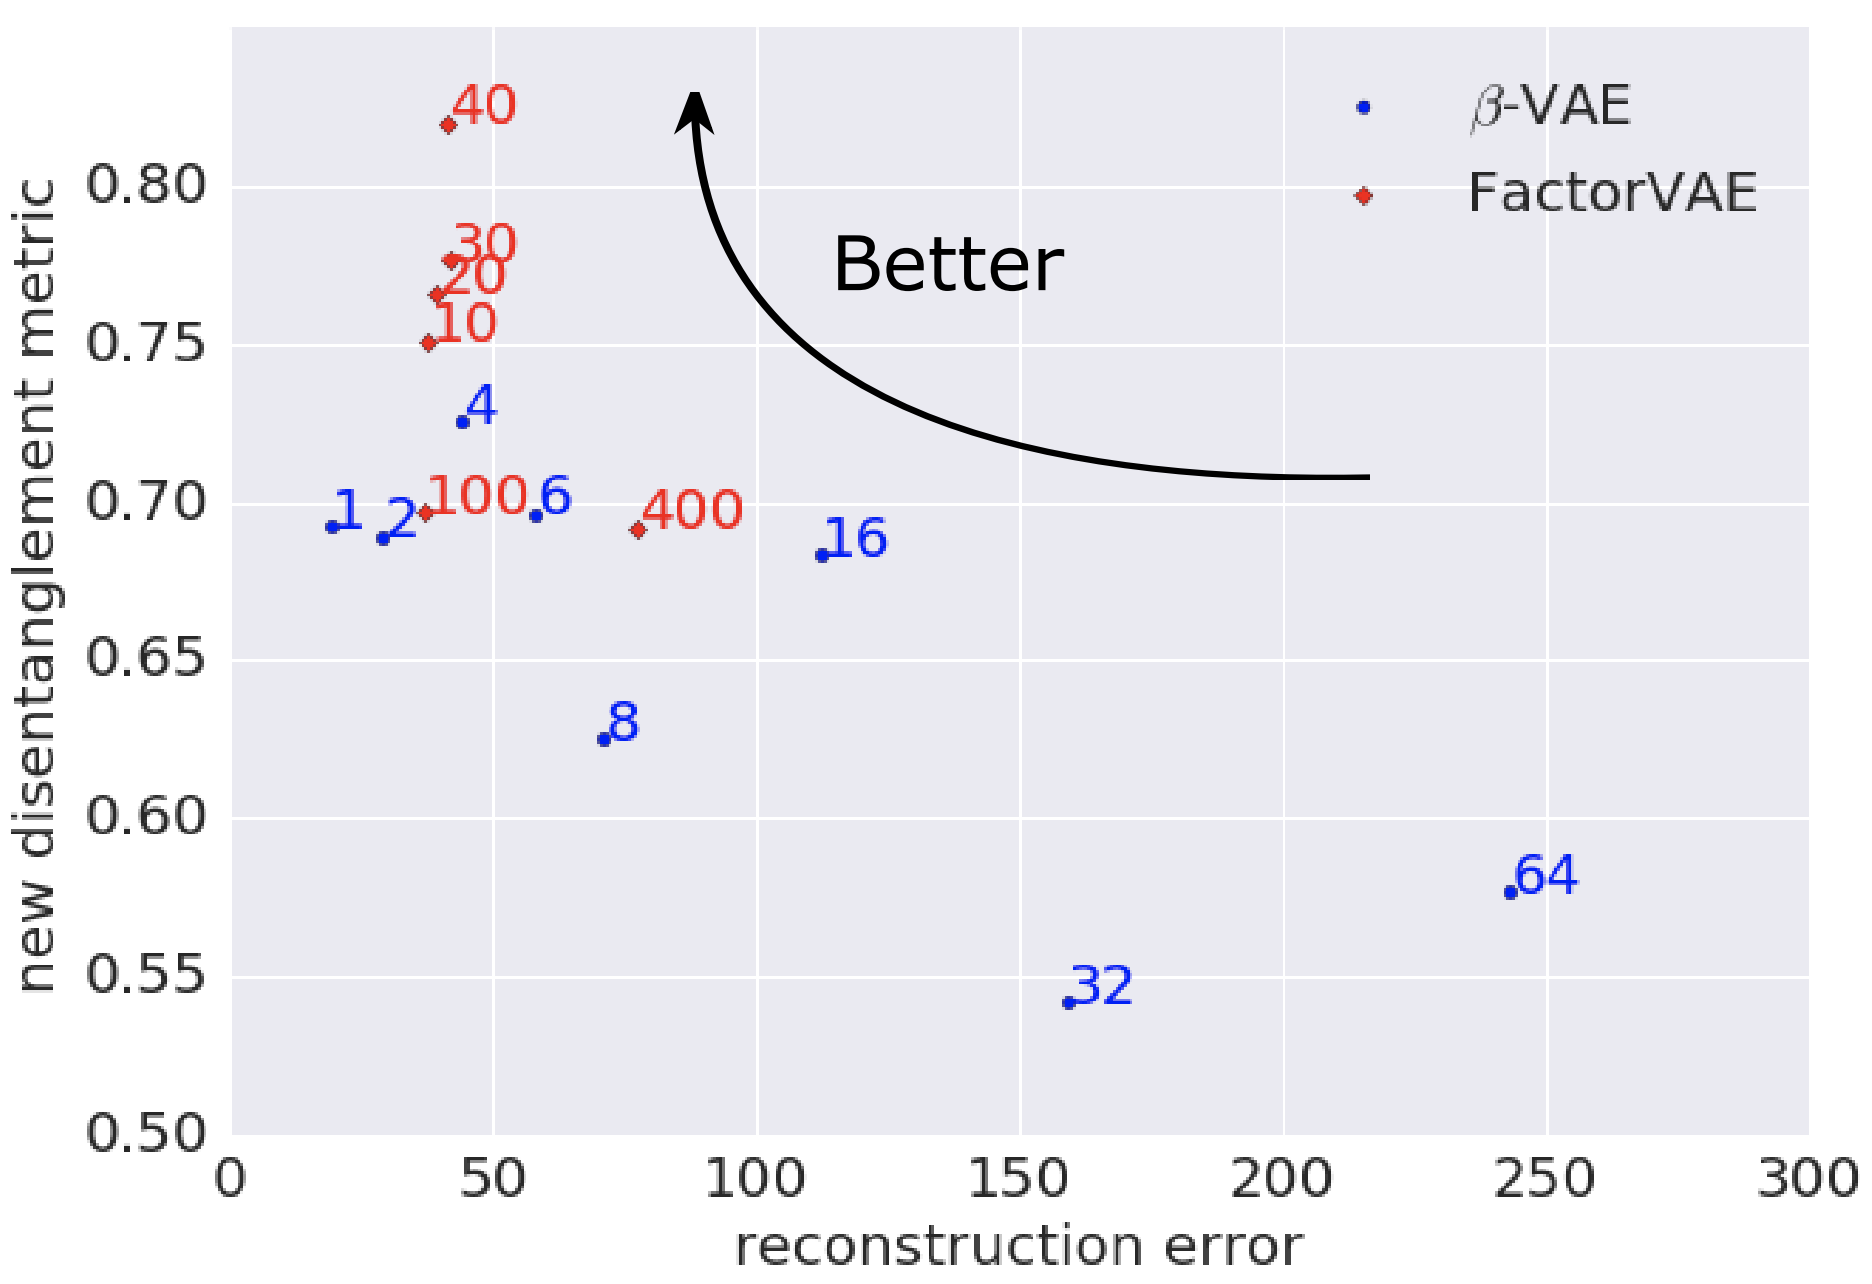
\includegraphics[width=\linewidth]{figs/factorvae_2}
		\end{figure}
	\end{minipage}

	\myfootnotewithlink{https://arxiv.org/abs/1802.05983}{Kim H., Mnih A. Disentangling by Factorising, 2018}
\end{frame}
%=======
\begin{frame}{Summary}
\begin{itemize}
	\item VampPrior proposes to use a variational mixture of posteriors as the prior to approximate the aggregated posterior.
	\vfill
	\item The autoregressive flows could be used as the prior. This is equivalent to the use of the IAF posterior. 
	\item More powerful decoder in VAE leads to more expressive generative model. However, too expressive decoder could lead to the posterior collapse.
	\item The decoder weakening is a set of techniques to avoid the posterior collapse.
\end{itemize}
\end{frame}
\end{document} 